%*******************************************************************************AAA
%*********************************** Chapter XXXXXXXX *****************************
%*******************************************************************************

\nomenclature[z-PoCA]{PoCA}{Point of Closest Approach} 

\chapter{Simulations of the DUNE Far Detector}  %Title of chapter
\graphicspath{{FarDetectorSimulations/Figs/Raster/}{FarDetectorSimulations/Figs/PDF/}{FarDetectorSimulations/Figs/Vector/}}

Previous work presented has been done concerning the 35 ton prototype, however it is also important to simulate the DUNE Far Detector (FD). Simulations in the FD have concentrated on cosmogenic background to neutrino oscillations, discussed in Section~\ref{sec:LBNESurf}, and the muon background to nucleon decay, discussed in Section~\ref{sec:DUNENDK}. The simulations shown in Section~\ref{sec:LBNESurf} are discussed in~\citep{MartinsThesis}, and were performed for the Long Baseline Neutrino Experiment (LBNE), which along with the Long Baseline Neutrino Oscillation (LBNO) experiment, formed the basis for DUNE, and so are included here for completeness. The author contributed by incorporating the \emph{complex} detector geometry, and the accurate surface profile, into the simulations, though the main body of work was performed by the author of~\citep{MartinsThesis}. The other work presented was performed for the DUNE collaboration, in conjunction with work done by Vitaly Kudryavtsev and Matthew Robinson, both of the University of Sheffield. This work was performed with the aim of producing muon-induced background limits to nucleon decay in the DUNE FD. \\

%********************************** %Second Section  **************************************
\section{Simulations of the LBNE surface detector} \label{sec:LBNESurf} %Section - X.2
A preliminary design of the LBNE experiment had a 10 kt LAr detector on the surface, with a 3 m rock overburden~\citep{LBNE6493}. Due to the large flux of cosmic rays at such a shallow depth, and the relative scarcity of neutrino events, it is necessary to establish whether the cosmic background can be sufficiently removed to allow neutrino interactions to be discerned. In order to show this, a series of simulations using both a simplified, and a more detailed detector design are performed. The cosmogenic backgrounds due to muons, protons and neutrons, are considered. These simulations, unlike other work presented in this thesis, were performed using a stand alone version of GEANT4, and not in LArSoft. For a more thorough review of the simulations, see~\citep{MartinsThesis}. \\

Simulations have been built using GEANT4 versions 9.4 and 9.6. Initial simulations were performed using version 9.4, before being rebuilt to use version 9.6. A study showing that the background rate did not change with the newer version of GEANT4 was performed, in order to verify that the two sets of simulations were consistent. In all simulations the physics list ``Shielding'' was used~\citep{Shielding}. Shielding is a well used physics list which includes extensive processes for a wide range of particles, with a large range of energies. \\

The simplified geometry, referred to as the \emph{simple} geometry, consisted of a single cuboid of LAr measuring 30 $\times$ 15 $\times$ 16 m$^3$. A representation of the \emph{simple} geometry is shown in Figure~\ref{fig:SurfSimpGeom}. The detector is enclosed in a flat layer of rock measuring 5 $\times$ 10$^3$ m in both the $x$ and $y$ directions. The rock has a depth of 22 m in the $z$ direction, including an overburden of 3 m. As simulations were not performed in LArSoft, the co-ordinate system used is defined as follows;
\begin{itemize}
\item $x$ - parallel to the beam direction.
\item $y$ - perpendicular to the beam direction.
\item $z$ - vertical direction.
\item The co-ordinate system is centred on the middle of the detector volume in $x$ and $y$, and on the surface of the rock in $z$.
\end{itemize}
The more detailed geometry, referred to as the \emph{complex} geometry, was a much more realistic detector design~\citep{LBNE3383}. The \emph{complex} geometry had two identical cryostats, each containing 120 TPC cells measuring 2.52 $\times$ 2.28 $\times$ 7.00 m$^3$. These cells each contain an active volume of LAr which measures 2.27 $\times$ 2.25 $\times$ 6.30 m$^3$. The TPC cells are arranged such that are 6, 10 and 2 TPC cells in the $x$, $y$ and $z$ directions, respectively. This gives a total volume of LAr in each cryostat which measures 28.20 $\times$ 13.95 $\times$ 15.0 m$^3$. Running vertically between the TPC cells are anode plane assemblies (APAs) and cathode plane assemblies (CPA's), all of which are embedded within the larger blocks of LAr. These blocks of LAr are further housed inside stainless steel containers, which are insulated by $0.8$ m of polyurethane. The two cryostats are shielded by $0.5$ m of concrete on all sides, with an additional $3$ m of concrete separating them. This gives a total fiducial mass of $10.7$ kton of active LAr, which is surrounded by additional LAr. A representation of the detector, produced by the GEANT4 visualisation tool, is shown in Figure~\ref{fig:SurfCompGeom}. \\

\begin{figure}[h!]
  \centering
  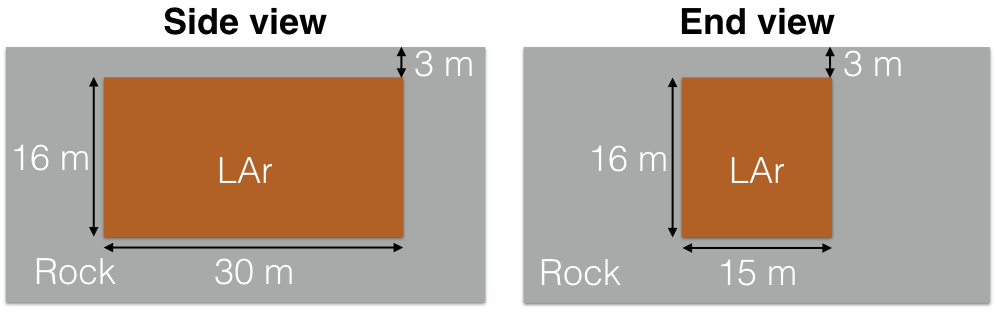
\includegraphics[width=\textwidth]{SimpleDetector}
  \caption[The \emph{simple} detector geometry used in the LBNE surface detector simulations]
          {The \emph{simple} detector geometry used in the LBNE surface detector simulations. Both a side view, and an end view is shown to scale. The rock is shown as a grey box. The active volume of LAr is shown as an orange box. The dimensions of the detector, and the overburden are shown in white around the active volume of LAr.}
  \label{fig:SurfSimpGeom}
\end{figure}

\begin{figure}[h!]
  \centering
  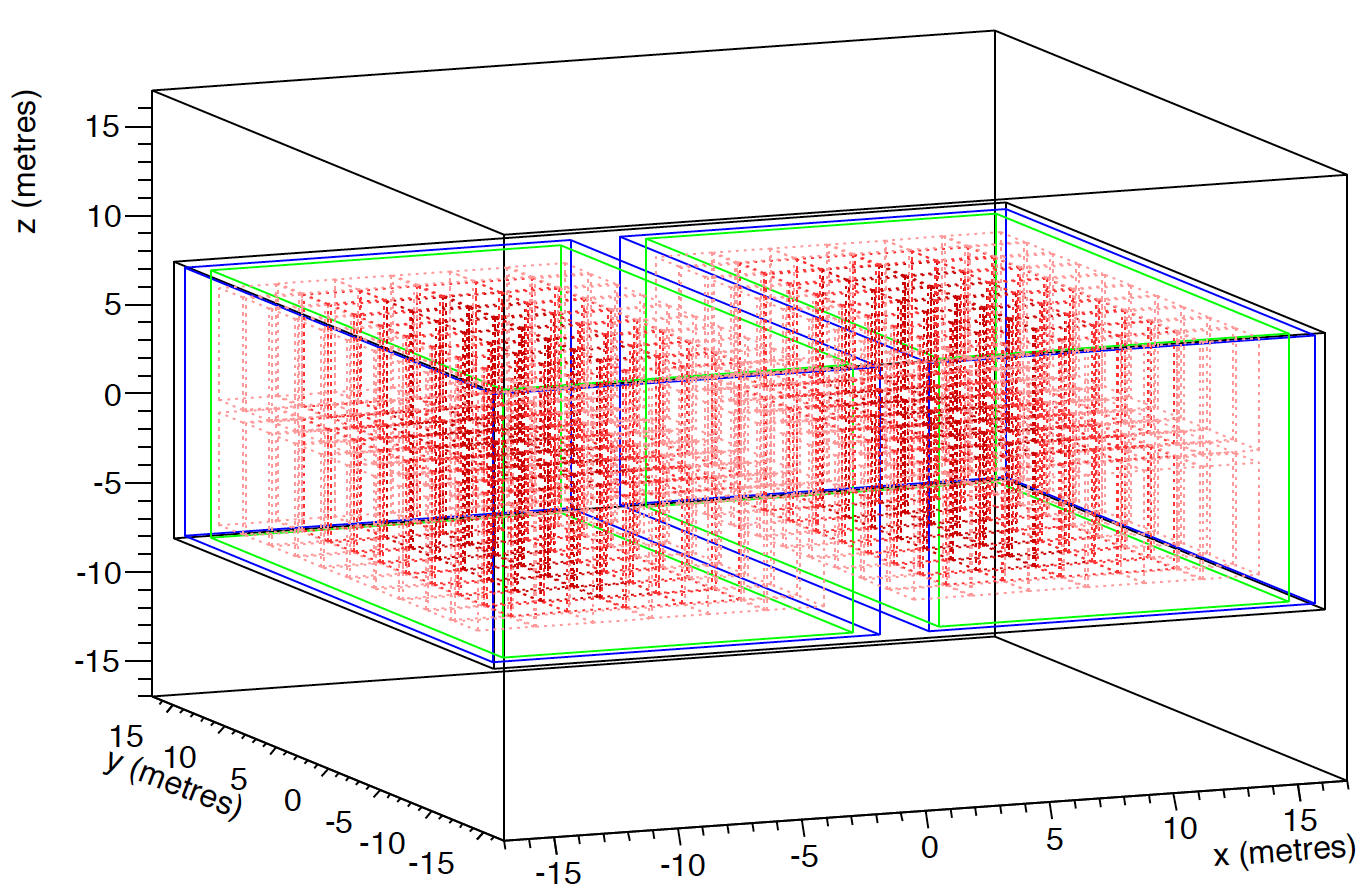
\includegraphics[width=0.8\textwidth]{ComplexGeom}
  \caption[The \emph{complex} detector geometry used in the LBNE surface detector simulations]
          {The \emph{complex} detector geometry used in the LBNE surface detector simulations. The TPC cells are shown in red, and are orientated such that are 9 $\times$ 6 $\times$ 2 in the $x$ $\times$ $y$ $\times$ $z$ co-ordinates, in each cryostat. The steel walls of the cryostats are green, whilst the outer edges of polyurethane are blue, and the concrete enclosures are black. Figure taken from~\citep{MartinsThesis}.}
  \label{fig:SurfCompGeom}
\end{figure}

The muons used in the simulations are generated using a Gaisser's parameterisation~\citep{Gaisser}, which has been modified for large zenith angles, and muon decay~\citep{PhysRevD.58.092005}. The protons and neutrons used in the simulations are generated using CRY~\citep{CRY,CRY2}, at an altitude of 2100 m. However, the LBNE surface detector would have had an altitude of 1505 m, and so the particle fluxes generated by CRY, have to be corrected to the particle fluxes expected at 1505 m. As the muon flux is calculated at sea level, this flux also has to be corrected so as to be the flux at 1505 m. The fluxes generated by CRY are also subject to a further correction, as CRY underestimates the cosmic ray flux by as much as 70\%~\citep{LBNE7517}. This is because CRY only considering protons striking the Earth's atmosphere. \\

Due to the large flux of cosmic ray particles at the surface, it is important to only simulate the particles which will cause background events. This is in order to reduce simulation time, and to reduce disk space. As such, if it can be seen that large portions of the cosmic fluxes do not induce background events, then these particle need not be simulated, and can instead can be accounted for through scaling of the simulated background. For example, it is found that 92.7\% of the proton induced background events are due to protons with energies of 10 GeV or more, yet these particles represent only 0.76\% of the total proton flux. This means that by not simulating protons with energies below 10 GeV, the vast majority of background events will be simulated, but this will require less than 1\% of the simulation time. The background events which are not simulated, can be accounted for by correcting the background seen from simulations, by the proportion of background events which were not simulated. For example, in the case of only simulating protons above 10 GeV, 7.3\% of the background were not simulated, and so the background rate from simulations should be scaled by a factor of 1.0787 $\left(\frac{1}{0.927}\right)$. Table~\ref{tab:SurfEnPrim} shows the minimum energies of the simulated muons, protons, and neutrons, along with the percentage of background events which they cause, and the percentage of the particle fluxes which particles of those energies, or more, represent. \\
\begin{table}[h!]
  \caption[The minimum energies of simulated particles, when determining the cosmogenic background for the LBNE surface detector]
          {The minimum energies of simulated particles, when determining the cosmogenic background for the LBNE surface detector. The percentage of background events which are caused by particles of these energies, or above, is shown. The percentage of the particle flux which has at least this much energy, is also shown. It can be seen that, with appropriate minimum energy constraints, it is possible to avoid simulating over 80\% of the muon flux, 99\% of the proton flux, and 95\% of the neutron flux.}
  \centering
  \label{tab:SurfEnPrim}
  \begin{tabular}{c c c c}
    \toprule
        {Primary particle} & {Min. energy simulated (GeV)} & {Background (\%)} & {Particle flux (\%)} \\ 
        \midrule
        Muons              & 10                            & 92.3              & 19.6                 \\

        Proton             & 10                            & 92.7              & 0.76                 \\

        Neutrons           & 1                             & 95.6              & 6.5                  \\
    \bottomrule
  \end{tabular}
\end{table}

\subsection{Description of cuts used} \label{sec:SurfCutList}
As noted above, the event rate due to cosmic backgrounds will be much larger than the neutrino event rate, and so a series of cuts, designed to remove cosmic background, whilst preserving signal events, have to be developed. This section will concern the cuts which were developed to achieve this. \\

The simplest cut considers the energy of the electromagnetic (EM) cascade which is induced. As is the case for DUNE, the LBNE beamline was a broadband neutrino beam, and had an energy range of between 0.25 and 5.0 GeV. This means that any EM cascade which deposited more than 5 GeV of energy into the detector could not be due to the interaction of a neutrino. A lower limit of 250 MeV is also applied, as the neutrinos in the beam will not have energies below this value. \\

Charged particles will leave a track in the detector, so it will be possible to identify whether a shower is caused by a charged particle entering the detector by extrapolating the particle tracks forwards, and backwards. Due to scattering, these extrapolated tracks will rarely cross perfectly, however many will have small track separations. Comparing the separation of these tracks at all points along the line, allows a minimum separation to be found, and if this is less than a pre-decided value, the shower can be identified as a background event. Figure~\ref{fig:SurfPoCACut} shows how this PoCA is calculated. It is found that imposing a $30$ cm point of closest approach (PoCA) cut with respect to the initial charged muon, should one enter the detector, removes a significant number of the background events which that muon may induce. A further PoCA cut of 10 cm, is then applied to all other charged particles, though tracks for which the PoCA is less than 2 cm are not removed. This is because it is possible that hadrons, such as a $\pi^{+}$, are produced at the neutrino interaction vertex, along with an $e^{+}$. An example of this interaction, along with a potential background source, is shown in Figure~\ref{fig:SurfSigBack}. In the example event shown in Figure~\ref{fig:SurfSigBack}, the PoCA between the $\pi^{+}$ and the $e^{+}$ would be much smaller than 10 cm, and the event is due to a neutrino interaction, therefore it should not be identified as a background event. A lower limit of 2 cm is used, as this represents 4 times the wire separation of the LBNE detector. It is assumed that should full reconstruction be performed, it would be able to resolve tracks to within this distance. \\

\begin{figure}[h!]
  \centering
  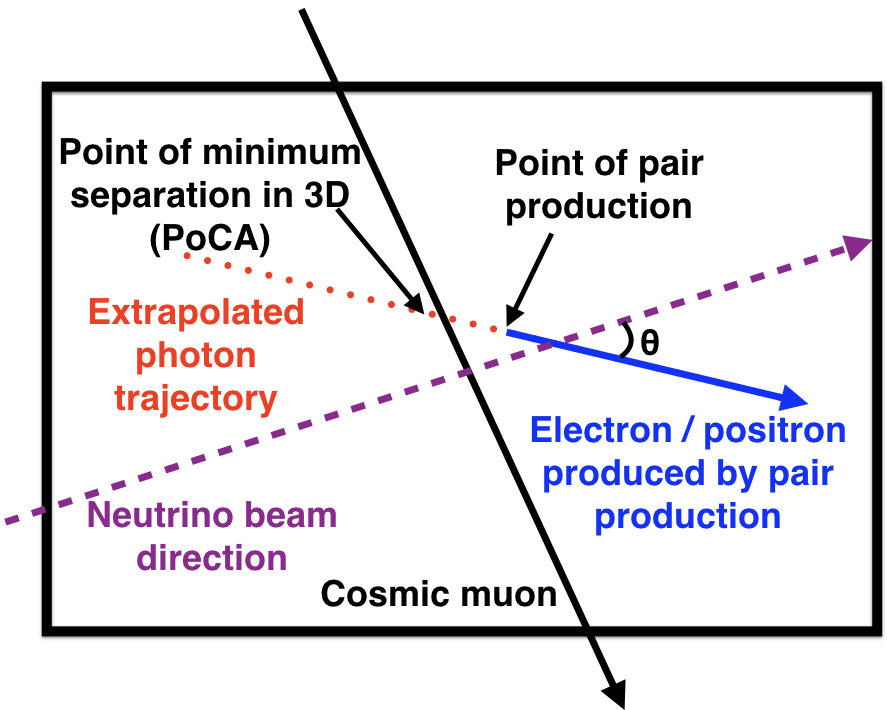
\includegraphics[width=0.6\textwidth]{PoCA_Beam_Cuts}
  \caption[How the PoCA, and the angle w.r.t the beam, cuts are calculated in the LBNE surface detector simulations]
          {How the PoCA, and the angle w.r.t the beam, cuts are calculated in the LBNE surface detector simulations. A cosmic muon which passes through the detector is shown as a black line, whilst an electron/positron that is produces is shown as a blue line. The minimum distance between the muon and electron/positron is shown (d), as well as the point of closest approach (PoCA) when the electron/positron track is extrapolated backwards. The extrapolated track is shown as a dotted red line. The neutrino beam direction is shown as a dashed green line, and the angle that the electron/positron makes with respect to this is shown ($\theta$).}
  \label{fig:SurfPoCACut}
\end{figure}

\begin{figure}[h!]
  \centering
  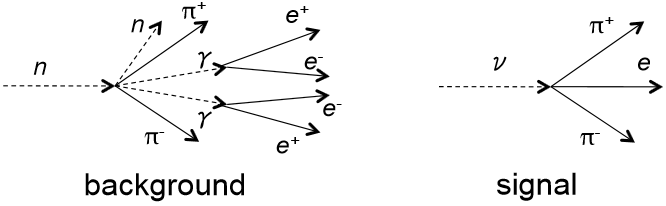
\includegraphics[width=0.6\textwidth]{signal_PoCA}
  \caption[An example of both a signal event, and a background event, where hadrons are produced at the interaction vertex]
          {An example of both a signal event, and a background event, where hadrons are produced at the interaction vertex. Left shows a potential background event induced by a neutron. It can be seen that two charged pions are produced, as well as two photons which will cause EM showers. Right shows a potential signal event, where there are also two pions produced at the interaction vertex, as well as an electron. The all charged PoCA calculated for both events will be very small, it is therefore possible that these two signals could be mistaken for each other. To prevent incorrectly assigning the signal event as a background event, any event with an all charged PoCA of less than 2 cm is not identified as a background event.}
  \label{fig:SurfSigBack}
\end{figure}

It has been found that the angle of a neutrino event, with respect to the neutrino beam, is highly correlated to the energy of the neutrino~\citep{barker2012muon}. This means that it is possible to use the angle of a shower, with respect to the beam, to distinguish between signal, and backgrounds events. Figure~\ref{fig:SurfPoCACut} shows how this angle is calculated, whilst Figure~\ref{fig:SurfBeamCut} shows that this cut is highly effective for high energy showers, as then the signal events will be tightly concentrated around the beam axis. This means that any high energy showers which are not tightly correlated to the beam axis will be identified as backgrounds~\citep{LBNE6621}. However, it also shows that the cut is much less effective for low energy showers, as the neutrino events are distributed over a large range of angles. The beam axis was imagined to be orientated at $6^\circ$ with respect to the horizon, and at an angle of $7^\circ$ with respect to West. This was to allow for the detector to be aligned along the line between Fermilab and the Homestake mine, given the Earth's curvature, and the local surface contours. \\

\begin{figure}[h!]
  \centering
  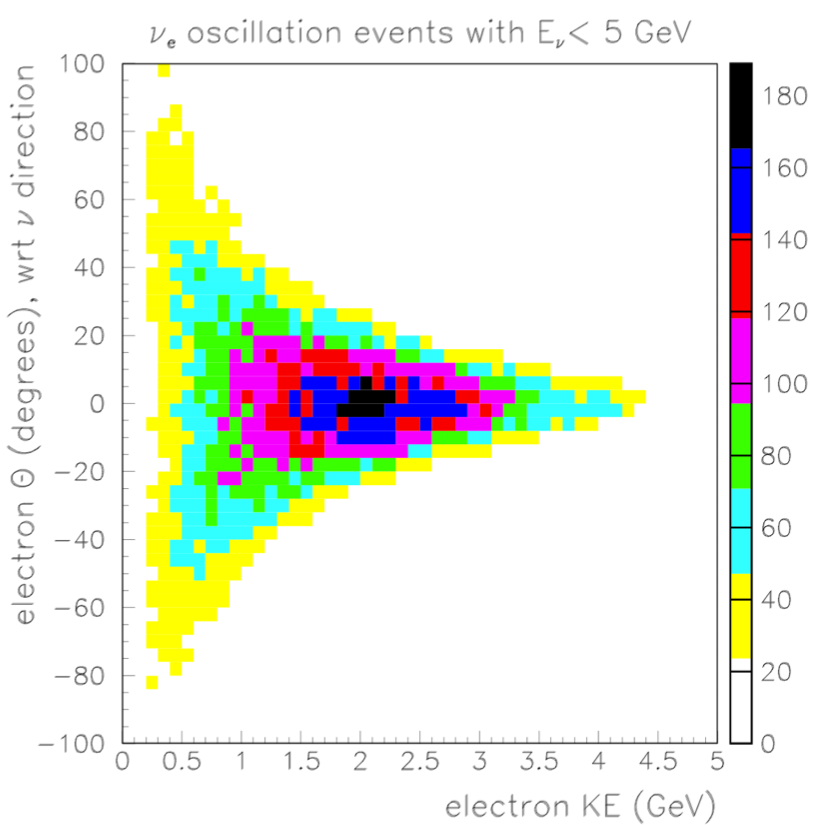
\includegraphics[width=0.6\textwidth]{SurfBeamCut}
  \caption[The energy dependence of the angle between the neutrino beam direction, and the electrons generated by simulated $\nu_{e}$ interactions]
          {The energy dependence of the angle between the neutrino beam direction, and the electrons generated by simulated $\nu_{e}$ interactions. An angular cut, given by the constraints of the plot, is used to reject background events where the angle of the electron/positron w.r.t the beam, does not match the expected energy spectrum for a signal event. Figure taken from~\citep{barker2012muon}.}
  \label{fig:SurfBeamCut}
\end{figure}

It is envisioned that not all of the instrumented LAr will be able to used to identify neutrino events. This is because, a fiducial cut will be applied around the detector edges, in order to ensure that the entire track is contained within the active volume of the detector. For the \emph{simple} detector this was simply a 30 cm cut around the edges of the active volume, however for the $complex$ detector, this fiducial cut is only applied to the outward facing edges of the active volumes. This is because it is assumed that tracks passing between cells, within a given cryostat, will be able to be stitched, as is done in LArSoft. \\

Additionally, signal events should be able to be distinguished from background events based on the energy deposition measurements. These will come from identifying the start of an EM shower as coming from either an electron, or a photon, in the case of a signal, and background event, respectively. External studies have shown that the failure rate of this separation tails off at 10\% for showers with energies above 0.5 GeV~\citep{LBNE8458}. Therefore, a flat reduction of $1/10$ is applied to all surviving simulated background events. \\

Finally, it is envisioned that an efficient photon detection system will be used, which uses the scintillation light emitted by excited argon~\citep{PhysRevB.27.5279}. This efficient photon detection system should be able to provide information on individual events, and so identify whether a candidate event occurred within the beam spill. If this is used, then the effective drift time of the detector can be reduced from 1400 $\mu$s to only 10 $\mu$s, a reduction by a factor of 140. This is also applied as a flat reduction to all surviving background events. \\

\subsection{Background with the \emph{simple} geometry, and flat surface profile}
A total of 2.7 $\times$ 10$^8$ muons, with energies greater than 10 GeV, are generated using the \emph{simple} detector geometry, and the flat surface profile. This represents 0.237 years worth of detector live time. Initially a total of 1.48 $\times$ 10$^8$ primary photons a year were observed, however, many of these were due to $\mu \rightarrow e \rightarrow \gamma$, and so as the first electron in the shower can be directly connected to an external charged particle, they will automatically be identified as background events. Events of this kind were removed from all subsequent simulations, and are not shown in any of the following tables. The number of events which survive the application of the cuts outlined in Section~\ref{sec:SurfCutList}, is shown in Table~\ref{tab:SurfMuSimp}. The errors quoted in Table~\ref{tab:SurfMuSimp}, and all subsequent tables in this section, are Gaussian, unless the annual rate drops to 0, meaning that no simulated particles survived the application of cuts. When this happens an upper limit, at 90\% confidence level~\citep{PhysRevD.57.3873}, is used, and any further scaling factors are applied to this upper limit. Errors are only quoted in the following tables if the error is more than 1\% of the annual rate. \\

\begin{table}[h!]
  \caption[The normalised annual background rate, for events where a primary muon enters the active volume of the detector, for the \emph{simple} geometry, and flat surface profile]
          {The normalised annual background rate, for events where a primary muon enters the active volume of the detector, for the \emph{simple} geometry, and flat surface profile. The background rate is separated into different first generation photon ancestries.}
  \label{tab:SurfMuSimp}
  \centering
  \scriptsize
  \begin{tabular}{l c c c c c c c c }
    \toprule
        & $E_\gamma$ & $PoCA_\mu$ & $\theta_{beam}(E)$ & $PoCA_{all}$ & $D$ $>$ $30$ cm & $e-\gamma(E)$ & $\gamma$ $detection$ \\
        \midrule
        $Total$          & $1.07\times10^7$ & $78500$    & $38400\pm500$ & $20400\pm400$ & $17700\pm400$ & $1770\pm34$ & $12.64\pm0.024$ \\

        $\pi^0\to\gamma$ & $2.27\times10^6$ & $78000$    & $38100\pm500$ & $20300\pm400$ & $17700\pm400$ & $1769\pm34$ & $12.64\pm0.024$ \\

        $Ext\to\gamma$   & $2.08\times10^6$ & $331\pm46$ & $159\pm32$    & $108\pm25$    & $0-15.53$     & $0-1.55$    & $0-0.010$ \\

        $\mu\to\gamma$   & $6.34\times10^6$ & $0-15.53$  & $0-7.59$      & $0-3.40$      & $0-2.96$      & $0-0.30$    & $0-0.002$ \\

        $Other\to\gamma$ & $2.84\times10^4$ & $172\pm33$ & $70\pm20$     & $0-15.53$     & $0-13.50$     & $0-1.35$    & $0-0.001$ \\
        \bottomrule
  \end{tabular}
\end{table}

From Table~\ref{tab:SurfMuSimp}, it can be seen the application cuts is very effective at removing the potential background events. The importance of achieving good electron/$\gamma$ separation, and the development of an efficiency photon detection system is plainly visible, as without these cuts, the background rate would be prohibitive to neutrino physics. Of the other cuts, the PoCA cut with respect to the initial muon entering the detector, is particularly effective, as it removes 99\% of the background events. If the PoCA cut is relaxed from a PoCA cut of 30 cm, to a PoCA cut of 10 cm, it is still found to remove 98.5\% of events. This shows how powerful this cut is. it is however, seen that the PoCA cut with respect to all charged particles is not as effective, though it still removes 47\% of background events. It is found that this is because proton hits were not stored in the simulations. In a sample of 0.017 years worth of statistics, where the proton hits are stored, the all charged particle PoCA cut is found to be more than 4 times as effective. If the all charged particle PoCA cut were seen to be this effective in the larger sample, this would mean that the annual background rate, after all cuts are applied, would be 2.84$\pm$0.41 yr$^{-1}$. This would be a significant improvement on when the proton hits are not saved. In all further simulations, proton hits are saved. \\

It is also necessary to consider events where the initial muon does not enter the detector, but still produces secondaries which enter the detector. The number of these events which mimic neutrino events, as successive cuts are applied, is shown in Table~\ref{tab:SurfMuMissSimp}. The PoCA cut with respect to the initial charged muon can obviously not be applied, as it does not enter the detector. For this reason, that cut is omitted from Table~\ref{tab:SurfMuMissSimp}, and all other tables not concerning muons which enter the active volume of the detector. \\

\begin{table}[h!]
  \caption[The normalised annual background rate, for events where a primary muon misses the active volume of the detector, for the \emph{simple} geometry, and flat surface profile]
          {The normalised annual background rate, for events where a primary muon misses the active volume of the detector, for the \emph{simple} geometry, and flat surface profile. The background rate is separated into different first generation photon ancestries.}
  \label{tab:SurfMuMissSimp}
  \centering
  \scriptsize
  \begin{tabular}{l c c c c c c c }
    \toprule
        & $E_\gamma$ &  $D$ $>$ $30$ cm & $\theta_{beam}(E)$ & $PoCA_{all}$ & $e-\gamma(E)$ & $\gamma$ $detection$ \\
        \midrule
        $Total$          & $10700\pm300$ & $770\pm70$ & $222\pm38$ & $159\pm32$ & $15.9\pm3.2$ & $0.11\pm0.02$ \\

        $\pi^0\to\gamma$ & $891\pm75$      & $433\pm52$ & $178\pm34$ & $115\pm27$ & $11.5\pm2.7$ & $0.08\pm0.02$ \\

        $Ext\to\gamma$   & $9802\pm249$  & $337\pm46$ & $45\pm17$  & $45\pm17$  & $4.5\pm1.7$  & $0.03\pm0.01$ \\

        $Other\to\gamma$ & $0-15.53$     & $0-1.22$   & $0-0.30$   & $0-0.23$   & $0-0.02$     & $0-0.0002$ \\
        \bottomrule
  \end{tabular}
\end{table}

From Table~\ref{tab:SurfMuMissSimp}, it can be seen that the overall background rate from muons which do not enter the active volume of the detector, is much less than the background from muons which enter the active volume of the detector. This is to expected, as many of these events are caused by external photons entering the detector, and when the fiducial cut is applied, a lot of these will be removed. It can also be seen that the angular beam cut is highly effective, removing 71\% of the background events, this is because there is no angular dependence on these events, and so other than the lowest energies, they can be reliably removed. \\ 

A sample of 1.06 $\times$ 10$^{7}$ neutrons, with energies above 1 GeV, were generated. This corresponds to a detector live time of 0.220 years. The number of events which mimic neutrino events, as successive cuts are applied, is shown in Table~\ref{tab:SurfNeuSimp}. \\

\begin{table}[h!]
  \caption[The normalised annual background rate, for neutron induced events, for the \emph{simple} geometry, and flat surface profile]
          {The normalised annual background rate, for neutron induced events, for the \emph{simple} geometry, and flat surface profile. The background rate is separated into different first generation photon ancestries.}
  \label{tab:SurfNeuSimp}
  \centering
  \scriptsize
  \begin{tabular}{l c c c c c c c }
    \toprule
        & $E_\gamma$ &  $D$ $>$ $30$ cm & $\theta_{beam}(E)$ & $PoCA_{all}$ & $e-\gamma(E)$ & $\gamma$ $detection$ \\
        \midrule
        $Total$          & $66900$       & $39700\pm500$ & $13900\pm300$ & $1725\pm95$ & $172.5\pm9.5$ & $1.23\pm0.07$ \\

        $\pi^0\to\gamma$ & $48500\pm500$ & $36600\pm400$ & $13100\pm300$ & $1569\pm90$ & $156.9\pm9.0$ & $1.12\pm0.06$ \\

        $Ext\to\gamma$   & $17100\pm300$ & $2348\pm110$  & $670\pm59$    & $156\pm28$  & $15.6\pm2.8$  & $0.11\pm0.02$ \\

        $Other\to\gamma$ & $1174\pm78$   & $888\pm68$    & $145\pm27$    & $0-12.67$   & $0-1.27$      & $0-0.009$ \\
        \bottomrule
  \end{tabular}
\end{table}

From Table~\ref{tab:SurfNeuSimp}, it can be seen that the predominant background from neutrons comes in the form of the $\pi^0\to\gamma$ channel. The relatively large number of events which survive all cuts, is due to the relative inefficiency of the fiducial cut, as it removes only 40\% of background events. This is because many of the $\pi^0\to\gamma$ events are deep within the LAr, because the neutron may interact deep within the active volume of the detector. When this occurs the $\pi^0$ will be produced a large distance away from the detector edges, and so will survive the fiducial cut. The fiducial cut is still seen to be effective at removing events which were caused by an external $\gamma$. The cut with respect to the angle of the beam, and the all charged PoCA cut, are both seen to be effective, removing 65\% and 88\% of the overall background respectively. \\

Finally, a sample of 10$^{8}$ protons, with energies above 10 GeV, have been generated. This corresponds to a detector live time of 0.270 years. The number of events which mimic neutrino events, as successive cuts are applied is shown in Table~\ref{tab:SurfProSimp}. \\

\begin{table}[h!]
  \caption[The normalised annual background rate, for proton induced events, for the \emph{simple} geometry, and flat surface profile]
          {The normalised annual background rate, for proton induced events, for the \emph{simple} geometry, and flat surface profile. The background rate is separated into different first generation photon ancestries.}
  \label{tab:SurfProSimp}
  \centering
  \scriptsize
  \begin{tabular}{l c c c c c c c }
    \toprule
        & $E_\gamma$ &  $D$ $>$ $30$ cm & $\theta_{beam}(E)$ & $PoCA_{all}$ & $e-\gamma(E)$ & $\gamma$ $detection$ \\
        \midrule
        $Total$          & $(1.05\pm0.06)\times10^{5}$ & $56100\pm500$ & $22100\pm300$ & $3601\pm115$ & $360.1\pm11.5$ & $2.57\pm0.08$ \\

        $\pi^0\to\gamma$ & $78100\pm500$               & $59600\pm500$ & $20600\pm300$ & $3335\pm110$ & $335.5\pm11.0$ & $2.38\pm0.08$ \\

        $Ext\to\gamma$   & $24500\pm300$               & $3477\pm112$  & $1138\pm64$   & $259\pm31$   & $25.9\pm3.1$   & $0.19\pm0.02$ \\

        $Other\to\gamma$ & $2393\pm93$                 & $2028\pm86$   & $390\pm38$    & $7.3\pm5.2$  & $0.73\pm0.52$  & $0.005\pm0.004$ \\
        \bottomrule
  \end{tabular}
\end{table}

From Table~\ref{tab:SurfProSimp}, it can be seen that the number of proton induced events is larger than the number of neutron induced events. This is true both for the initial number of events, and the number of events which survive the application of cuts. This is despite the charged nature of the proton meaning that it interacts more readily with the surrounding rock, and will create a track with which a PoCA cut can be made with respect to, should the proton enter the LAr. The application of the fiducial cut is seen to be relatively ineffective, removing only 38\% of the background events, though it is very effective at removing events in the $Ext\to\gamma$ channel. The all charge PoCA is observed to be very effective, as would be expected, where it removes 84\% of the background events. However, even after all cuts a very substantial 2.57 $\pm$ 0.08 events per year survive the application of all cuts. \\

This results in a total of 16.55 $\pm$ 0.26 events per year surviving the application of all cuts, when background events from muons entering the active volume of the detector, muon missing the active volume of the detector, neutron induced events, and proton induced events, are counted. This figure is reduced to approximately 5 events, when the effect that including proton hits in the muon simulations is accounted for. It is interesting to consider the effect that considering an accurate surface profile, and a \emph{complex} detector geometry, will have on the number of background events which survive the application of all cuts. \\

\subsection{Background with the \emph{complex} geometry, and accurate surface profile}
It is prudent to observe the effect that the additional shielding found in the \emph{complex} geometry has on the background rate. The overall effect of the shielding is that there is roughly an extra metre of rock overburden, once the various stopping powers are summed. However, there is a roughly 10\% increase in fiducial mass, and most importantly, the surface area of the detector is substantially increased. It is thought that the additional shielding will have the effect of reducing the flux of particles entering the detector, though this may be different for muons which miss the active volume of the detector. The increased surface area means that is more chance that particles will enter the detector though, and the gaps between the TPC cells may have a very significant effect on the number of muons which do not enter the active volume of the detector, but still produce secondaries which enter the active volume of the detector. The reason for this, is that, with the presence of vertical gaps between TPC cells, it is possible for a vertical muon to pass undetected through the centre of the detector, and to then produce secondaries which will be detected. Events such as this, will, at fist glance at least, appear very similar to a neutrino event, as they will be isolated in the centre of the detector. It is not known, which of these changes will have the largest effect on the overall background rate. \\

It is also prudent to observe the effect that including an accurate surface profile around the proposed detector site, has on the predicted background rates. The proposed location of the LBNE detector was the same as the proposed DUNE detector location, though it was on the surface, and not in the mine. A satellite generated map, centred on SURF, which encompasses an area of 20 $\times$ 20 km$^2$ is used to generate the accurate surface profile. The map is sampled in bins measuring 5 $\times$ 5 m$^2$. To include the effects that the surrounding hills would have on the muon flux, muons are initially sampled 600 m above the surface, and are then stepped through the surface profile, until they reach a box surrounding the detector, which measures 80 $\times$ 80 $\times$ 36 m$^3$.  The amount of rock which a muon passes through is calculated as it is stepped through the map, and the energy losses which this will cause are then taken into account before subsequent simulations. By taking the surface profile into account in this way, simulation time can be reduced by not having to simulate the surface profile for every new set of muons. This is because, the box upon which muon positions are stored is large enough to include the detector, plus a few metres of rock on all sides, to allow for muon cascades to develop. The surface profile is modified so as to have a flat surface above the detector location of 100 $\times$ 100 m$^2$. As this is the area upon which protons and neutrons are sampled, the effect of the accurate surface profile on their fluxes is assumed to negligible. The accurate surface profile is shown in Figure~\ref{fig:SurfProf_Col}. \\

Before the accurate surface profile was incorporated, a study was performed to measure the effect that using the \emph{complex} geometry, with the flat surface profile, would have on the expected background rate. The background rates found for both the \emph{simple} and \emph{complex} geometries, using the flat surface profile, are shown in Table~\ref{tab:SimpSurfRates}. \\

\begin{table}[h!]
  \caption[The expected rates for both the \emph{simple} and \emph{complex} detector geometries, using the flat surface profile]
          {The expected rates for both the \emph{simple} and \emph{complex} detector geometries, using the flat surface profile. The rates for muons entering the detector, muons missing the detector, proton induced events, and neutron induced events are shown. For the \emph{simple} detector geometry, the effect of including hits due to protons in the all PoCA cut is also shown, they are included by default in the \emph{complex} detector geometry.}
  \centering
  \label{tab:SimpSurfRates}
  \begin{tabular}{c c c c}
    \toprule
        {Primary particle} & {\emph{simple}, no proton hits} & {\emph{simple}, w. proton hits} & {\emph{complex}} \\ 
        \midrule
        Muons entering     & 12.64 $\pm$ 0.24                & $\sim$1.18                      & 1.94 $\pm$ 0.23  \\

        Muons missing      & 0.11 $\pm$ 0.02                 & 0.11 $\pm$ 0.02                 & 0.58 $\pm$ 0.14  \\

        Protons            & 2.57 $\pm$ 0.08                 & 2.57 $\pm$ 0.08                 & 0.23 $\pm$ 0.01  \\

        Neutrons           & 1.23 $\pm$ 0.07                 & 1.23 $\pm$ 0.07                 & 0.16 $\pm$ 0.01  \\

        Total              & 16.55 $\pm$ 0.26                & $\sim$5                         & 2.91 $\pm$ 0.27  \\
    \bottomrule
  \end{tabular}
\end{table}

From Table~\ref{tab:SimpSurfRates}, it can be seen that the background rate for the \emph{complex} detector is lower than for the \emph{simple} detector geometry. This is largely due to the additional shielding which is present in the \emph{complex} detector geometry, as it will significantly reduce the number of proton and neutron induced events. However, the extra shielding appears to have little effect on the muon rates both entering, and missing, the active volume of the detector. This is to be expected, as the stopping length for muons is much longer than that of hadrons, and the surface area of the detector has increased significantly as the geometry has been changed. The increase in surface area of the detector, along with the increase in mass, explains the increase in background observed for muons entering the active volume of the detector. Similarly, the background due to muons missing the active volume of the detector is affected by the increased surface area, and mass, but also by the presence of the gaps between TPC cells. This means that the effective surface area for muons missing the active volume of the detector is significantly increased. \\

Table~\ref{tab:SurfMuComp}, shows the background rate for muons which enter the active volume of detector, as sequential cuts are applied, for the \emph{complex} geometry, and accurate surface profile. A total of 2 $\times$ 10$^8$ muons, with energies greater than 10 GeV, are generated, representing 0.1003 years worth of detector live time. When comparing Table~\ref{tab:SurfMuComp}, with Table~\ref{tab:SurfMuSimp}, it can be seen that the overall number of background mimicking events increases when using the \emph{complex} detector geometry, and the accurate surface profile. The effect that including proton hits has on the effectiveness of the all charged particle PoCA cut is also clearly visible, as it removes many more background events when proton hits are saved. When comparing the rates seen for the \emph{complex} detector geometry in the flat, and accurate surface profile, it can be seen that the rates are consistent. This means that including the accurate surface profile, does not have a significant effect on the background rate. \\

\begin{table}[h!]
  \caption[The normalised annual background rate, for events where a primary muon enters the active volume of the detector, for the \emph{complex} geometry, and accurate surface profile]
          {The normalised annual background rate, for events where a primary muon enters the active volume of the detector, for the \emph{complex} geometry, and accurate surface profile. The background rate is separated into different first generation photon ancestries.}
  \label{tab:SurfMuComp}
  \centering
  \scriptsize
  \begin{tabular}{l c c c c c c c c }
    \toprule
        & $E_\gamma$ & $PoCA_\mu$ & $\theta_{beam}(E)$ & $PoCA_{all}$ & $D$ $>$ $30$ cm & $e-\gamma(E)$ & $\gamma$ $detection$ \\
        \midrule
        $Total$          & $1.32\times10^7$ & $(6.38\pm0.09)\times10^4$ & $(2.87\pm0.06)\times10^4$ & $3796\pm229$ & $2854\pm199$ & $285\pm20$   & $2.03\pm0.14$ \\

        $\pi^0\to\gamma$ & $2.24\times10^6$ & $(5.82\pm0.09)\times10^4$ & $(2.62\pm0.06)\times10^4$ & $3339\pm215$ & $2743\pm195$ & $274\pm20$   & $1.96\pm0.14$ \\

        $Ext\to\gamma$   & $4.48\times10^6$ & $5237\pm270$              & $2425/pm183$              & $457\pm80$   & $111\pm39$   & $11.1\pm3.9$ & $0.08\pm0.03$ \\

        $\mu\to\gamma$   & $6.36\times10^6$ & $0-34$                    & $0-15.20$                 & $0-2.01$     & $0-1.51$     & $0-0.15$     & $0-0.001$ \\

        $Other\to\gamma$ & $7.87\times10^4$ & $333\pm68$                & $97\pm37$                 & $0-15.20$    & $0-11.43$    & $0-0.11$     & $0-0.002$ \\
        \bottomrule
  \end{tabular}
\end{table}

The background rate for the \emph{complex} detector geometry, and accurate surface profile, for muons which miss the active volume of the detector, is shown in Table~\ref{tab:SurfMuMissComp}. The same muons used in Table~\ref{tab:SurfMuComp}, are used here, meaning that a detector live time of 0.1003 years is been simulated. When comparing the overall background for the \emph{complex} geometry, and accurate surface profile, to the background for the \emph{complex} geometry, and flat surface profile, shown in Table~\ref{tab:SimpSurfRates}, it can be seen the background rate after the application of all cuts, is unchanged by the inclusion of the accurate surface profile. It is found that the total background rate for the \emph{complex} geometry, before cuts are applied, is 10\% lower when using the accurate surface profile. This is expected, as the addition of hills will provide some addition shielding from muons at large angles. It would however, appear that these background events are largely removed through the application of cuts, as the background rate after the application of cuts, is unaffected by the inclusion of the accurate surface profile. \\

\begin{table}[h!]
  \caption[The normalised annual background rate, for events where a primary muon misses the active volume of the detector, for the \emph{complex} geometry, and accurate surface profile]
          {The normalised annual background rate, for events where a primary muon misses the active volume of the detector, for the \emph{complex} geometry, and accurate surface profile. The background rate is separated into different first generation photon ancestries.}
  \label{tab:SurfMuMissComp}
  \centering
  \scriptsize
  \begin{tabular}{l c c c c c c c }
    \toprule
        & $E_\gamma$ &  $D$ $>$ $30$ cm & $\theta_{beam}(E)$ & $PoCA_{all}$ & $e-\gamma(E)$ & $\gamma$ $detection$ \\
        \midrule
        $Total$          & $19800\pm500$ & $4004\pm235$ & $1551\pm147$ & $914\pm113$ & $91\pm11$      & $0.65\pm0.08$ \\

        $\pi^0\to\gamma$ & $3284\pm213$  & $1108\pm123$ & $526\pm85$   & $166\pm48$  & $16.63\pm4.80$ & $0.12\pm0.03$ \\

        $Ext\to\gamma$   & $16500\pm500$ & $2858\pm199$ & $998\pm118$  & $748\pm102$ & $75\pm10$      & $0.53\pm0.07$ \\

        $Other\to\gamma$ & $28\pm5$      & $28\pm5$     & $28\pm5$     & $0-20$      & $0-2.01$       & $0-0.01$ \\
        \bottomrule
  \end{tabular}
\end{table}

As illustrated earlier, the accurate surface profile was modified so as to have a flat 100 $\times$ 100 m$^{2}$ plane directly above the detector, where it is envisioned that the detector outbuildings would be. As such, the expected backgrounds for protons and neutrons are the same as was shown in Table~\ref{tab:SimpSurfRates}, as these particles were sampled on a plane measuring 100 $\times$ 100 m$^{2}$. Table~\ref{tab:SurfNeuComp}, and~\ref{tab:SurfProComp}, show the expected background rates, as sequential cuts are applied for the \emph{complex} detector geometry, and accurate surface profile, for neutrons and protons, respectively. Table ~\ref{tab:SurfNeuComp} is made from a total of 1.1 $\times$ 10$^8$ simulated neutrons, representing a detector live time of 0.653 years. Table~\ref{tab:SurfProComp} is made from a total of 1 $\times$ 10$^7$ protons, representing a detector live time of 2.482 years. As discussed when considering Table~\ref{tab:SimpSurfRates}, the reduced background rates seen in Tables~\ref{tab:SurfNeuComp} and~\ref{tab:SurfProComp}, when compared to Tables~\ref{tab:SurfNeuSimp} and~\ref{tab:SurfProSimp}, are due to the additional shielding in the \emph{complex} geometry. \\

\begin{table}[h!]
  \caption[The normalised annual background rate, for neutron induced events, for the \emph{complex} geometry, and flat surface profile]
          {The normalised annual background rate, for neutron induced events, for the \emph{complex} geometry, and flat surface profile. The background rate is separated into different first generation photon ancestries.}
  \label{tab:SurfNeuComp}
  \centering
  \scriptsize
  \begin{tabular}{l c c c c c c c }
    \toprule
        & $E_\gamma$ &  $D$ $>$ $30$ cm & $\theta_{beam}(E)$ & $PoCA_{all}$ & $e-\gamma(E)$ & $\gamma$ $detection$ \\
        \midrule
        $Total$          & $8405\pm113$ & $5697\pm93$ & $1949\pm54$  & $225\pm18$   & $22.5\pm1.8$  & $0.16\pm0.01$ \\

        $\pi^0\to\gamma$ & $6397\pm98$  & $5050\pm87$ & $1744\pm51$  & $194\pm17$   & $19.4\pm1.7$  & $0.14\pm0.01$ \\

        $Ext\to\gamma$   & $1796\pm52$  & $470\pm26$  & $169\pm16$   & $30.1\pm6.7$ & $3.01\pm0.67$ & $0.021\pm0.005$ \\

        $Other\to\gamma$ & $209\pm18$   & $175\pm16$  & $36.2\pm7.4$ & $0-3.68$     & $0-0.37$      & $0-0.003$ \\
        \bottomrule
  \end{tabular}
\end{table}

\begin{table}[h!]
  \caption[The normalised annual background rate, for proton induced events, for the \emph{complex} geometry, and flat surface profile]
          {The normalised annual background rate, for proton induced events, for the \emph{complex} geometry, and flat surface profile. The background rate is separated into different first generation photon ancestries.}
  \label{tab:SurfProComp}
  \centering
  \scriptsize
  \begin{tabular}{l c c c c c c c }
    \toprule
        & $E_\gamma$ &  $D$ $>$ $30$ cm & $\theta_{beam}(E)$ & $PoCA_{all}$ & $e-\gamma(E)$ & $\gamma$ $detection$ \\
        \midrule
        $Total$          & $1.55\times10^4$ & $10559\pm$ & $3475\pm39$ & $319\pm12$ & $31.9\pm1.2$ & $0.23\pm0.01$ \\

        $\pi^0\to\gamma$ & $1.18\times10^4$ & $9277\pm63$  & $3098\pm36$ & $297\pm11$ & $29.7\pm1.1$ & $0.21\pm0.01$ \\

        $Ext\to\gamma$   & $3120\pm37$      & $858\pm19$   & $279\pm11$  & $22\pm3$   & $2.2\pm0.3$  & $0.016\pm0.002$ \\

        $Other\to\gamma$ & $524\pm15$       & $424\pm15$   & $97\pm6$    & $0-1.04$   & $0-0.10$     & $0-0.001$ \\
        \bottomrule
  \end{tabular}
\end{table}

This gives the expected background for the \emph{complex} detector geometry, and accurate surface profile of 3.07 $\pm$ 0.25 events per year. The distribution of EM shower energies that this background represents is shown in Figure~\ref{fig:SurfEDistCuts}. This compares with the expected background rate of 16.65 $\pm$ 0.27 events per year, for the \emph{simple} detector geometry, and flat surface profile, when proton hits are not included in simulations, or $\sim$5 events per year when protons hits are saved. \\

\begin{figure}[h!]
  \centering
  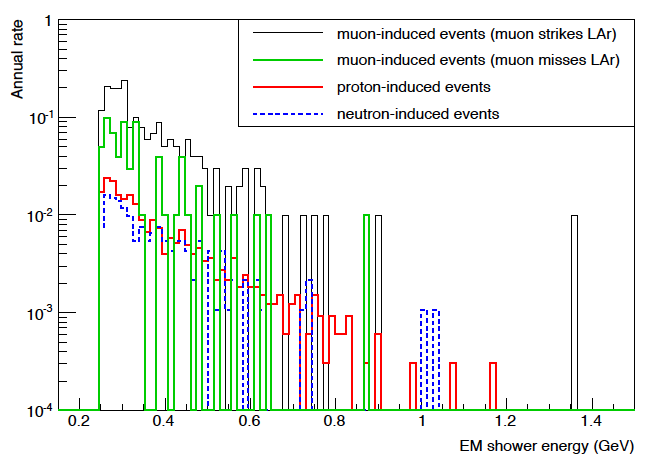
\includegraphics[width=0.6\textwidth]{SurfEDistAllCuts}
  \caption[The annual rate of cosmic background events, for different particles, as a function of the EM shower energy]
          {The annual rate of cosmic background events, for different particles, as a function of the EM shower energy. The annual rates events for background events induced by, muons striking the active volume, missing the active volume, protons, and neutrons, is shown. The background rates are for the \emph{complex} detector geometry, and accurate surface profile.}
  \label{fig:SurfEDistCuts}
\end{figure}

\subsection{Summary of simulations for the LBNE surface detector}
Following the simulation of large samples of muons, protons, and neutrons, with both a \emph{simple} and \emph{complex} detector geometry, the expected background for the LBNE surface detector is found when considering both a flat, and an accurate, surface profile. It is observed that the effect of the \emph{complex} detector geometry is to reduce the overall background rate, primarily due to the additional shielding which it provides. This additional shielding causes the proton and neutron induced backgrounds to decrease substantially, as was shown in Table~\ref{tab:SimpSurfRates}. It is however found that there will be a significant source of backgrounds from muons which do not enter the active volume of the detector. This is due to the large surface area of the detector design, and the presence of vertical gaps between the TPC cells. The effect of incorporating the accurate surface profile is found to be negligible, as the hills only offer minimal amounts of shielding. It was however, still very instructive to show this, and provides a complete and robust simulation of the expected background for the LBNE surface design. \\


%********************************** % Third Section  *************************************
\section{The use of MUSUN in LArSoft} \label{sec:FDIncorporation}  %Section - X.3
The primary muons in the following discussions are all generated using MUSIC~\citep{MUSUN}~\citep{MUSIC}~\citep{MUSIC2} and MUSUN~\citep{MUSUN}~\citep{MUSUN2}, and so a brief overview of them is required. MUSIC first propagates muons through a medium, defined by the user, for given initial energies, positions, and direction cosines. A range of energies between 10$^2$ and 10$^7$ GeV are considered, and their energy distributions are stored at depths of between 100 and 15,000 m w.e. Energy losses due to four processes are considered; ionisation, bremsstrahlung, electron-positron pair production and muon-nucleus inelastic scattering. The output of MUSIC is then used by MUSUN to generate a muon energy spectrum and angular distribution, for a given detector location. MUSUN is able to use information about the local surface profile to make these distributions more accurate. \\

The location of the DUNE far detector, near the Ross shaft at SURF, has global coordinates of, 44$^{\circ}$20$'$45.21$''$ North, 103$^{\circ}$45$'$16.13$''$ West. The rock composition is assumed to be, $< Z >$ = 12.09 and $< A >$ = 24.17. The density is assumed to be 2.70 g cm${-3}$~\citep{Mei:2009py}. The flux calculated by MUSIC/MUSUN of 5.18 $\times$ 10$^{-9}$ cm$^{-2}$ s$^{-1}$ sr$^{-1}$, is well matched to the flux measured by the active veto system of the Davis' experiment, which was (5.38 $\pm$ 0.07) $\times$ 10$^{-9}$ cm$^{-2}$ s$^{-1}$ sr$^{-1}$~\citep{PhysRevD.27.1444}. Given the small differences in these values, and another measurement by the Majorana demonstrator, the systematic uncertainty in calculating the muon flux is estimated to be 20\%~\citep{NDKTFNote}. \\

The surface profile around the proposed detector location is shown in Figure~\ref{fig:SurfProf_Col}, where the proposed location is in the centre of the map. Each quadrant on the map has been divided into 4 angles of 22$^{\circ}$, to help guide the eye when comparing it to Figure~\ref{fig:SurfProf_Azi}, where the distribution of azimuth angles is plotted. The vertical lines in Figure~\ref{fig:SurfProf_Azi} show the division of the quadrants when the angle is calculated from East to the North. When moving from East to North it is possible to discern how the peaks and troughs on the surface profile, correspond to troughs and peaks, in the distribution of azimuthal angle. \\

\begin{figure}[h!]
  \centering
  \begin{subfigure}{0.45\textwidth}
    \centering
    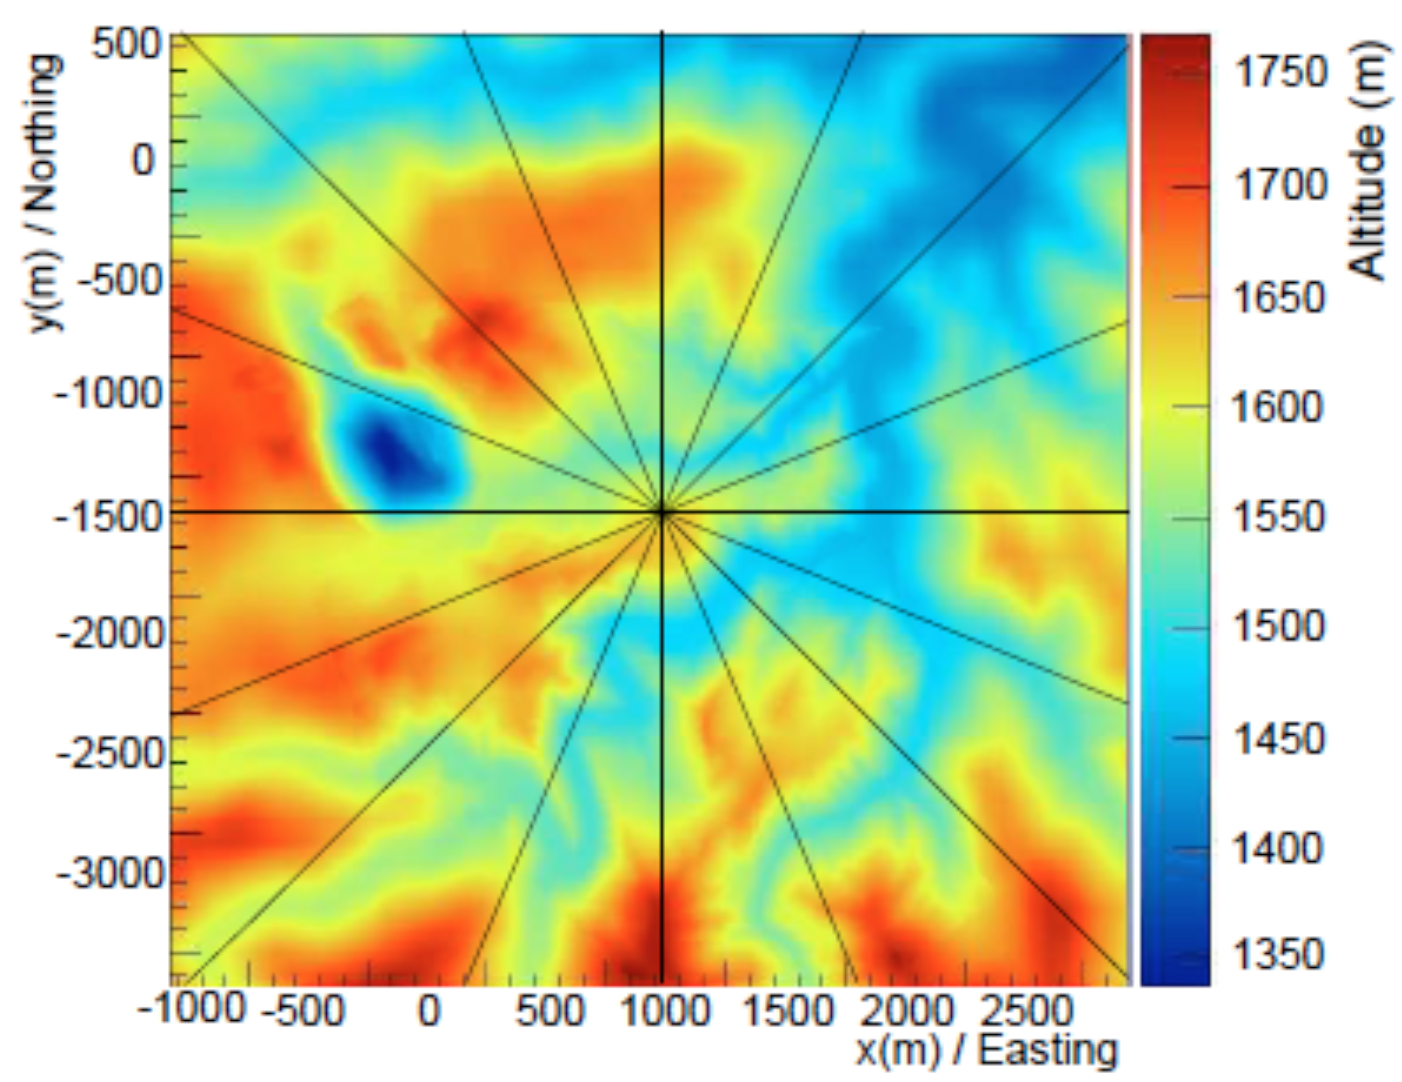
\includegraphics[width=\textwidth]{dune-surface-map}
    \caption{The surface profile of the DUNE far detector site at SURF.}
    \label{fig:SurfProf_Col}
  \end{subfigure}
  \hspace{0.08\textwidth}
  \begin{subfigure}{0.45\textwidth}
    \centering
    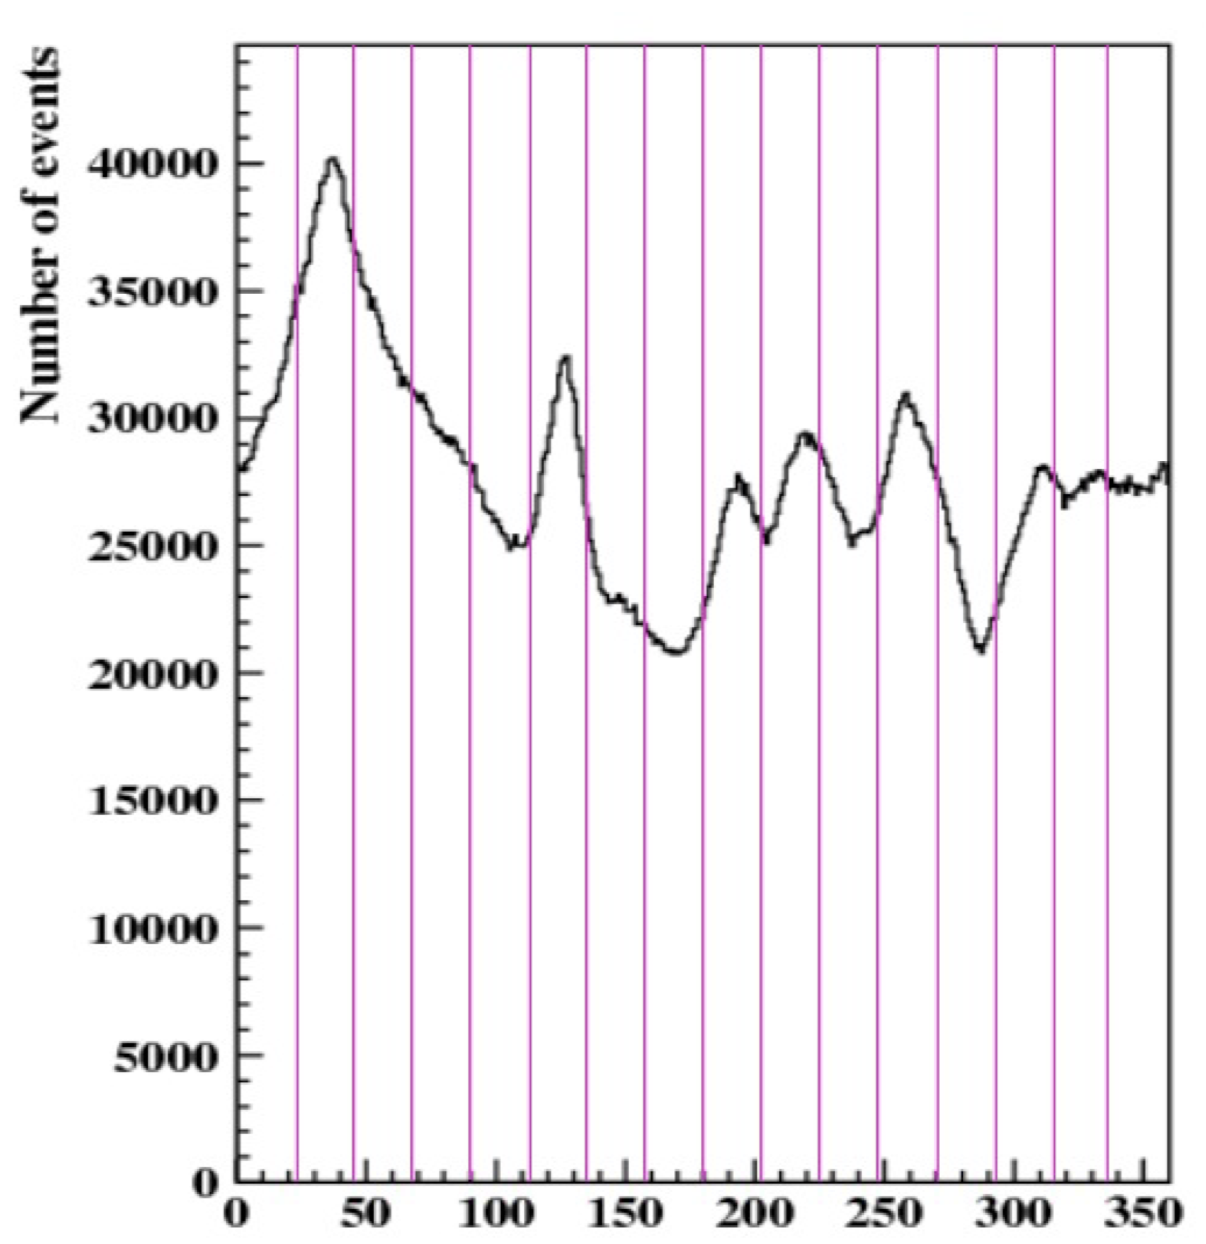
\includegraphics[width=\textwidth]{phi-map}
    \caption{The distribution of azimuthal angles of muons at the DUNE far detector site at SURF.}
    \label{fig:SurfProf_Azi}
  \end{subfigure}
  \caption[The correlation between the surface profile, and the distribution of azimuthal angles at the DUNE far detector site]
          {The correlation between the surface profile, and the distribution of azimuthal angles at the DUNE far detector site. The quadrants have been divided into four angles of equal size. The azimuthal angle, calculated as the angle from East (pointing to the right in Fig.~\ref{fig:SurfProf_Col}), and increasing counterclockwise, is seen to follow the contours of the surface profile.}
\end{figure}

Given these parameters, the muon flux at the DUNE far detector location, when assuming a spherical detector geometry, and without simulating a detector cavern, is given by Table~\ref{tab:MUSUNflux}. \\
\begin{table}[h!]
  \caption[Muon flux parameters as calculated with MUSIC/MUSUN.]
          {Muon flux parameters as calculated with MUSIC/MUSUN.}
  \centering
  \label{tab:MUSUNflux}
  \begin{tabular}{c c c c}
    \toprule
        {Total flux (cm$^{-2}$ s$^{-1}$)} & {Mean E$_{\mu}$ (GeV)} & {Mean slant depth (m w.e)} & {Mean $\theta$ ($^{\circ}$)} \\ 
        \midrule
        5.66 $\times$ 10$^{-9}$           & 283                    & 4532                       & 26                           \\
    \bottomrule
  \end{tabular}
\end{table}

The muons simulated for DUNE are sampled on the surface of a box surrounding the detector hall, that also encompasses 7 m of rock above the cavern, and 5 m of rock on all other sides. This is to ensure that the simulated muons pass through a sufficient amount of rock to induce cascades, both above, and around, the detector hall. The secondaries produced in these cascades which enter the detector, in the absence of the initial muon, are of particular interest, as they could be mistaken for nucleon decay events. The study of these nucleon decay mimicking events is discussed in Section~\ref{sec:DUNENDK}. The size of the box which the muons are sampled from is 74.43 $\times$ 29.54 $\times$ 30.18 m$^3$, compared to the simulated cryostat which has dimensions, 61.62 $\times$ 14.94 $\times$ 13.58 m$^3$. The dimensions are given as length $\times$ width $\times$ height. The muons are sampled randomly according to their energy spectrum, for a given zenith and azimuthal angle, using the angular distribution obtained with MUSIC. \\

Before this could be done however, MUSUN had to be incorporated into the DUNE software framework, as it had previously been maintained in FORTRAN, as an external package. This involved building on the work done by the LZ collaboration in porting the code to C++~!!!!!citep{Kareem}. The process by which this was done, was to first reproduce the distributions produced by the LZ collaboration using the DUNE software framework. Once the distributions could be reproduced for the Davis shaft at SURF (the proposed location of LZ), the muon distributions produced by the original FORTRAN code for the DUNE detector location were reproduced. The distributions produced by the DUNE software framework are shown in Figure~\ref{fig:MUSUNIncorp}. These are seen to be consistent with the distributions made for the LBNE collaboration~\citep{MUSUNLBNE}. The initial positions of 10,000 muons, generated in LArSoft around the simulated DUNE 10 kt module, are shown in Figure~\ref{fig:10ktPos}. The initial positions of the muons are shown as blue points, whilst the cryostat is a single black box, and each TPC is a single red box. \\

\begin{figure}[h!]
  \centering
  \begin{subfigure}{0.45\textwidth}
    \centering
    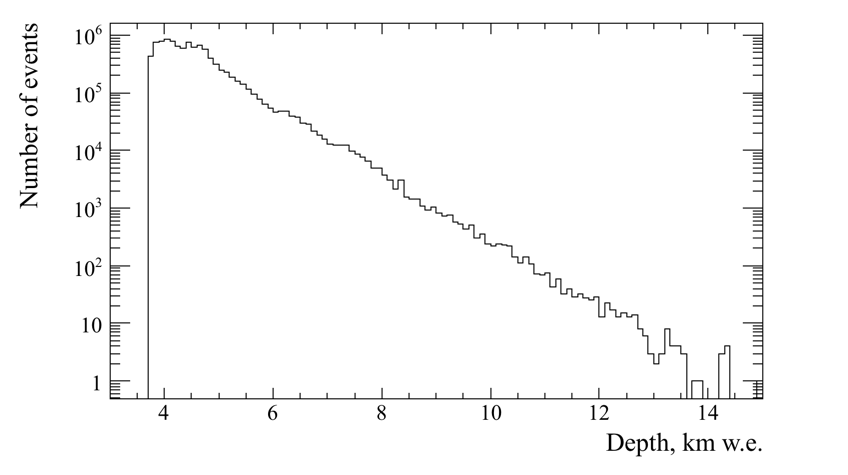
\includegraphics[width=\textwidth]{DepthCan}
    \caption{The number of muons with given slant depths.}
  \end{subfigure}
  \hspace{0.08\textwidth}
  \begin{subfigure}{0.45\textwidth}
    \centering
    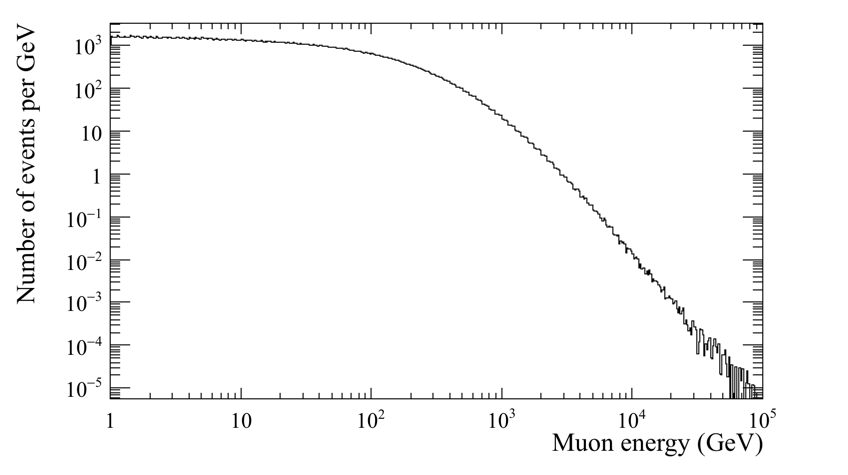
\includegraphics[width=\textwidth]{EnergyPerGeVCan}
    \caption{The initial energy spectrum of simulated muons.}
  \end{subfigure}
  % ========
  \begin{subfigure}{0.45\textwidth}
    \centering
    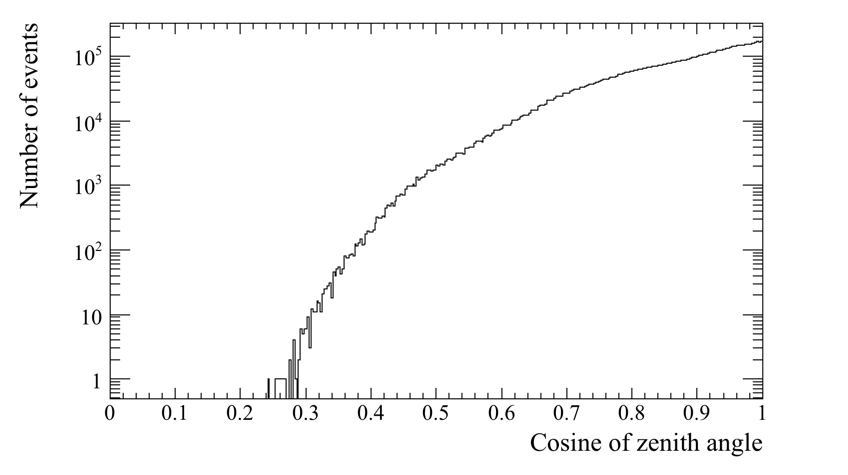
\includegraphics[width=\textwidth]{ZenithCan}
    \caption{The number of muons with given zenith angles.}
  \end{subfigure}
  \hspace{0.08\textwidth}
  \begin{subfigure}{0.45\textwidth}
    \centering
    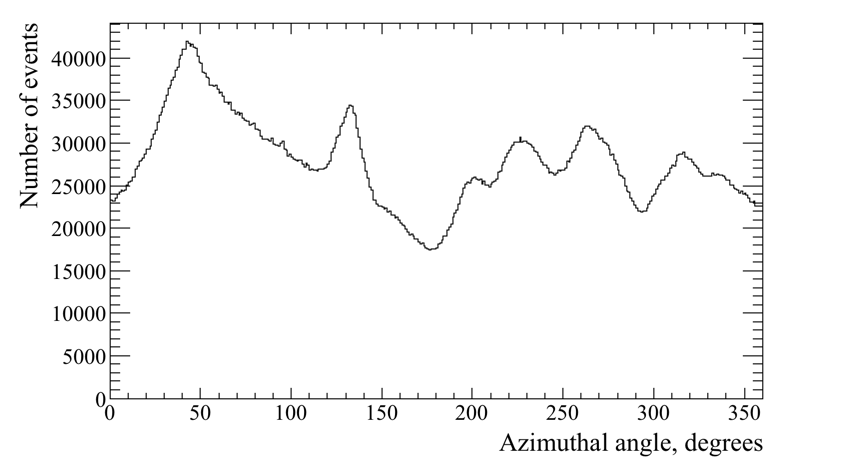
\includegraphics[width=\textwidth]{AzimuthCan}
    \caption{The number of muons with given azimuthal angles.}
  \end{subfigure}
  % ========
  \begin{subfigure}{0.45\textwidth}
    \centering
    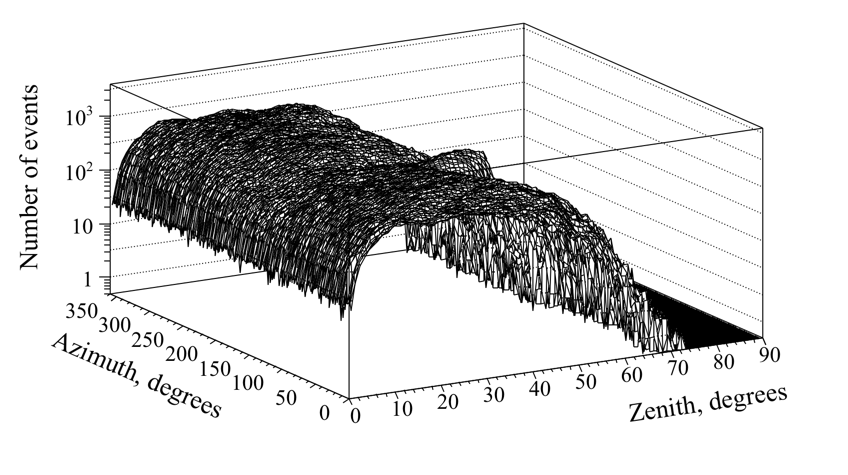
\includegraphics[width=\textwidth]{AziZenCan}
    \caption{The distribution of zenith and azimuthal angles.}
  \end{subfigure}
  \hspace{0.08\textwidth}
  \begin{subfigure}{0.45\textwidth}
    \centering
    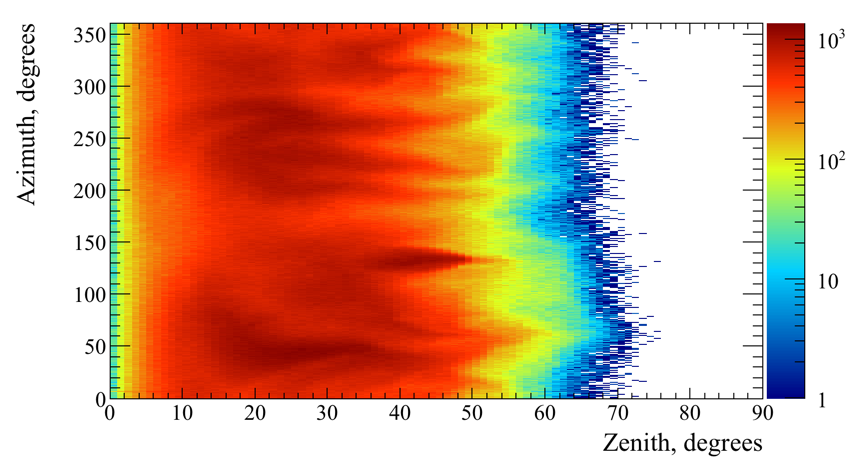
\includegraphics[width=\textwidth]{AziZenColzCan}
    \caption{The distribution of zenith and azimuthal angles, shown with a colour $z$ scale.}
  \end{subfigure}
  \caption[The distributions of some of the important quantities for a sample of 10$^6$ muons generated by MUSUN, in LArSoft]
          {The distributions of some of the important quantities for a sample of 10$^6$ muons generated by MUSUN, in LArSoft. The slant depths and energies of the simulated muons are shown top. The azimuthal and zenith angles of muons are shown middle. Bottom left shows the profile of zenith angle, against azimuthal angle, whilst bottom right shows this with a colour $z$ axis.}
  \label{fig:MUSUNIncorp}
\end{figure}

\begin{figure}[h!]
  \centering
  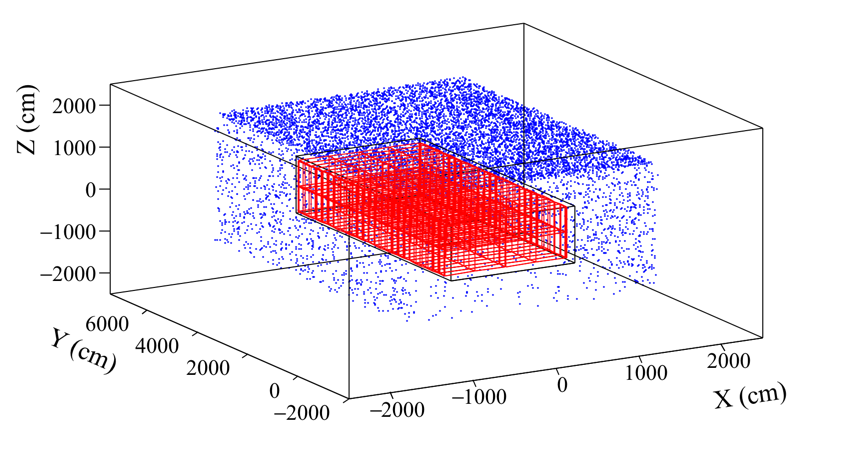
\includegraphics[width=\textwidth]{MuonPosCan}
  \caption[The initial positions of muons generated by MUSUN, around a DUNE 10 kt module]
          {The initial positions of muons generated by MUSUN, around a DUNE 10 kt module. The initial positions of the muons are shown as blue points, whilst the cryostat is a single black box and each TPC is a single red box.}
  \label{fig:10ktPos}
\end{figure}

It is found that the muon rate through the box upon which the muons are sampled is 0.1579 Hz. This rate is later used to normalise the background event rate in Section~\ref{sec:DUNENDK}. Roughly a third of the muons which are generated pass through the active volume, to give a muon rate through the active volume of 0.053 Hz. \\ 

%********************************** % Fifth Section  *************************************
\section{Nucleon decay channels in DUNE} \label{sec:DUNENDK} %Section - X.5
When searching for rare processes, where an experiment is unlikely to see more than a few real signatures, an exhaustive study of the potential backgrounds is required. This is so that if a signal is observed, it could provide overwhelming evidence for the process. The search for nucleon decay in DUNE is one such process, and so an exhaustive study of the background to nucleon decay is required. As discussed in Section~\ref{sec:BkNDK}, cosmogenic muons cause backgrounds to nucleon decay signatures, as the secondary particles produced by their interactions are able to mimic the nucleon decay signatures. For this reason it is necessary to simulate this background, and to develop a series of cuts which can be applied to the energy depositions they produce, to establish that they are not due to nucleon decays. When doing this, it is important to use a simulation that is as accurate as possible to the DUNE far detector. It is for this reason that MUSUN was incorporated into LArSoft, as the muons which it generates are well matched to the observed muon flux, as described in Section~\ref{sec:FDIncorporation}. \\

To ensure that the background has been properly simulated it is advantageous to simulate many more background events than will be collected by the experiment. As the DUNE detector will run for roughly 20 years, it was decided that an initial sample representing 200 years of detector live time would be simulated. Given that the muon rate through the cavern is 0.1579 Hz, 200 years of detector live time corresponds to roughly 10$^9$ muons. This only represents one of the DUNE 10 kt modules, and so an even larger dataset will be required to represent the full live time of the 4 10 kt modules. For this reason, muons were generated beyond this initial sample size, with a total of 2$\times$10$^9$ muons having been currently simulated. \\

Producing samples of this size requires significant computer power, both in terms of running time, and storage space. As such, many of the simulated events are discarded before being saved to disk. This is done through the application of a filter after GEANT4. It is essential that the events which are discarded could not have been mistaken for nucleon decay events, and so only very generous cuts are applied. Only events satisfying one of the following cuts are discarded;
\begin{itemize}
\item Contain a muon track of more than 1 m.
\item There are no energy depositions in the entire detector volume.
\end{itemize}
It is envisioned that a muon track of more than a metre would not be unreconstructed. It is also assumed that any signatures observed within one drift window of such a track would not be studied in a nucleon decay search, as there would be doubt as to the authenticity of the signal. Given that the total rate of muons through the active volume is 0.053 Hz, and that the drift time is a few ms, ignoring all times where any track from a cosmogenic muon is present results in less than 0.1\% dead time. The dead time associated with ignoring events with muon tracks of more than 1 m is clearly less than this. This amount of dead time is assumed to be acceptable. Filtering out events where there are no energy depositions in the detector is clearly acceptable, as there are no energy depositions which could mimic a nucleon decay signature. \\

After applying this series of cuts, the sample of 2$\times$10$^9$ muons is reduced to XXXX$\times$10$^{XXXX}$ muons, which is a much more reasonable sample size to store on tape, and to perform analyses on. It is upon this reduced sample of muons that the cosmogenic background analyses are performed. As discussed in Section~\ref{sec:DUNE_NDK}, the proton decay channel of $p \rightarrow K^{+} + \bar{\nu^{e}}$ is referred to as the 'Golden Channel' in LAr, this analysis is discussed in~\citep{NDKTFNote}. The related decay of channel of $n \rightarrow K^{+} + e^{-}$ is discussed here. \\

%********************************** % Fifth.First Section  *************************************
\subsection{Cosmogenic background to the $n \rightarrow K^{+} + e^{-}$ decay channel} \label{sec:NDKCosmBk}
As shown in Table~\ref{tab:NDKLim}, the predicted sensitivity that DUNE will have to this channel is much larger than that of Super-K. As a result, it is an interesting decay mode to study as DUNE could easily have the best limit for this decay channel. As discussed in Section~\ref{sec:BkNDK}, the cosmogenic background to nucleon decay is predominantly caused by neutral particles, such as a $K^0$, entering the detector volume, and interacting far away from the detector edges. This is particularly true for the 'Golden Channel,' as shown in Figure~\ref{fig:K0LongBackground}, but it also holds for other channels. This means that it is events such as this which are the main cause for concern when trying to eliminate all cosmogenic backgrounds. \\

As is the case with the 'Golden Channel,' the final state of the decay contains a single charged kaon, and so events which do not contain a kaon track can be immediately discounted. There is also an electron in the final state of the decay, and so this means that events which do not also contain an electron can be discounted. In a nucleon decay event, the kaon and electron produced in the final state will have a common vertex, and so the requirement that the two particles have a common vertex can also be applied. Other constraints that are applied to eliminate background events are; a cut on external muon length, a cut on depositions near the detector edges, and criteria about the distribution of deposited energy. The criteria about the distribution of deposited energy is found by considering a sample of simulated decay events, and is discussed in Section~\ref{sec:NDKEnCosmBk}. These cuts, which are applied sequentially, are outlined below:
\begin{itemize}
\item The event contains energy depositions due to kaons and due to electrons.
\item The event contains at least one kaon track, and at least one electron track/shower.
\item The event contains a single kaon track, and a single electron track/shower.
\item No muon travels more than 20 cm in the detector volume.
\item The event has no energy depositions within 2 cm of the detector edges.
  \begin{itemize}
  \item This is changed to a maximum of 100 MeV of energy deposited within 2 cm of the detector edge in Section~\ref{sec:NDKSig}.
  \end{itemize}
\item The kaon and electron share a common vertex.
  \begin{itemize}
  \item The kaon and electron tracks are separated by no more than 5 cm.
  \item If the kaon and electron tracks are separated by more than 5 cm, then the point of closest approach between the two extrapolated tracks is less than 2 cm.
  \end{itemize}
\item The energy depositions in the event are within the ranges expected from a nucleon decay event. This is explained in Section~\ref{sec:NDKEnCosmBk}, but the energies considered are summarised below:
  \begin{itemize}
  \item The energy directly deposited by the kaon.
  \item The energy deposited by the kaon decay products.
  \item The energy directly deposited by the electron.
  \item The energy deposited near the shared kaon and electron vertex.
  \item The energy deposited in the detector which does not fit any of the above criteria.
  \end{itemize}
\end{itemize}
Inspiration for these cuts were taken from~\citep{Bueno}, though some of the cuts were relaxed. The cut on muons was relaxed from a cut on any muon being present, to a maximum track length of 20 cm, as this was found to be sufficient. The cuts on the number of pions in the event were relaxed so as to not expect that all particles are perfectly reconstructed. However, as the analysis is performed using Monte Carlo truth information, without position or energy smearing, the kaons and electrons are assumed to be perfectly reconstructed. This means that it is assumed that all deposited charge will be reconstructed, and that the detector characterisation is perfect. This is something which will need to be refined in future analyses, and will be taken into account when the analysis progresses to use reconstructed quantities, as discussed in Section~\ref{sec:NDKImprov}. \\ 

When performing the analysis it is important to be able to trace the particle ancestry. This is so that energy depositions in the detector can be properly assigned, and cuts applied, to the relevant particles. For example, a $\mu^{+}$ is often produced when a $K^{+}$ decays at rest, and this muon may travel more than 20 cm. However, the cut on muon length should not be applied to this muon as it was produced by the decay of the kaon. Similarly, as the kaon interacts in the detector secondary particles will be produced, which will be reconstructed as tracks coming off the main kaon track. The initial kinetic energy of the kaon can only be determined by summing the energy depositions due to these secondary particles, and the energy depositions due to the kaon itself. Correctly calculating the initial kaon kinetic energy is critical when determining if an event is a nucleon decay event. The reason for this is that nucleon decay events have very specific energy spectra, and so being able to correctly assign the ancestry of energy depositions is vitally important. The same is true for the electron energy, which is calculated by tracing the ancestry of the particles produced in the EM shower which it produces back to the electron. \\

As no reconstruction has been performed, the tracks referred to here are different from those in previous sections. The definition of a track used here, is that the particle in question has energy depositions, on simulated wires, which are directly associated with it. These simulated wires are not the same as the the wires which have been considered in previous Monte Carlo studies, as the signals have not been digitised. This distinction is important, as it allows the energy depositions directly from GEANT4 to be used, whilst also allowing for LArSoft methods concerning whether depositions are within TPC boundaries to be utilised. \\

The simulated electrons may begin showering immediately, or they may produce a short 'track like' segment before beginning to shower. To ensure that every electron shower can be identified, electrons are not required to produce a short 'track like' segment. This means that all electrons are assumed to begin showering immediately, and it is also assumed that all of the energy in the shower can be identified as coming from a single electron. This definition of shower energy is the one that is used when the showering algorithms are developed in LArSoft. It is hoped that when DUNE begins taking data the showering algorithms will be able to achieve this level of energy reconstruction. \\

When calculating the distance between the start of the kaon track, and the start of the electron track/shower, the energy depositions whose locations are closest to the Monte Carlo truth start points of the particles are used. For particles which are produced within the active volume, these locations generally correspond to the Monte Carlo truth start positions, though this is not always the case. For example, if a particle is created in the gap between two TPCs, then there will be no charge collected until it enters the active volume. This will result in the measured start position to be shifted from the true generation point. This shift can prove troublesome when considering decay events, as if the decay occurred in the centre of an APA, then it is likely that the kaon and electron would deposit energy on opposite sides of the APA. This would cause the depositions to be separated by over 5 cm, as this is the width of the APAs. However, if the tracks are propagated backwards, towards their true start point, it should still be possible to determine that they had a common vertex. An example of a simulated decay event where this happens is shown in Figure~\ref{fig:NDK_Sig_KEBigGap}. \\

\begin{figure}[h!]
  \centering
  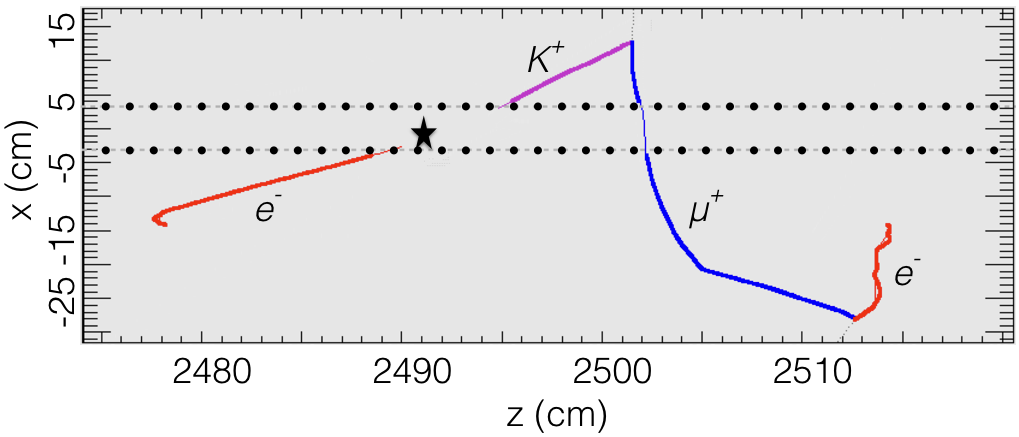
\includegraphics[width=0.8\textwidth]{KaonElecBigGap}
  \caption[A simulated $n \rightarrow K^{+} + e^{-}$ decay which occurred in a gap between TPCs]
          {A simulated $n \rightarrow K^{+} + e^{-}$ decay which occurred in a gap between TPCs. The path of the kaon produced in the decay is shown as a purple line. The path of the muon, produced by the decay of the kaon, is shown as a blue line. The paths which the electrons in the event took are shown as red lines. The electron on the left of the figure is the electron produced in the neutron decay, whilst the one on the right of the figure, is produced by the decay of the muon. The thin coloured lines show track segments which were in uninstrumented parts of the detector, such as gaps between TPCs and APAs. The dotted black lines show the edges of the TPCs, and the black star shows the location at which the decay occurred. The distance between the first kaon energy deposition, and the first electron energy deposition, is found to be 10.7 cm. However, when the kaon and electrons tracks are extrapolated towards the true start position, the point of closest approach (PoCA) between the two tracks is found to be 0.67 cm. This shows that they do in fact have a common vertex, despite the large separation of the start points.} 
  \label{fig:NDK_Sig_KEBigGap}
\end{figure}

In order for a kaon track, and an electron shower, to be considered to share a common vertex, the separation between the start of the kaon track, and the start of the electron shower, must be no more than than 5 cm. A maximum separation of 5 cm is used, as, if the two particles are produced in the centre of a TPC, a gap of 5 cm would require no energy depositions to be collected over approximately 10 collection wires. This is assumed to be unlikely during data taking, and cannot happen in the simulations considered here, as Monte Carlo truth information is used. As shown by Figure~\ref{fig:NDK_Sig_KEBigGap}, however, it is possible for the kaon and electron, produced in a signal event, to be separated by more than 5 cm. To prevent events such as this being missed, a second criteria is applied to events with large separations. This criteria is that the ``Point of Closest Approach'' (PoCA) between the two particles, found by extrapolating the kaon track and the electron shower, forwards and backwards, is less than 2 cm. This is the same PoCA calculation which was made in Section~\ref{sec:SurfCutList}, and it means that events such as the one shown in Figure~\ref{fig:NDK_Sig_KEBigGap} are still identified as signal events. \\

The fiducial cut is only applied to the outer edges of the cryostat, as if it were done with respect to the edge of every TPC in the far detector the loss of volume would be prohibitive. This means that the event shown in Figure~\ref{fig:NDK_CosmoBack_Raw} would not fail the fiducial cut, as the decay occurred over 6 m away from the edge of the detector, but happened to be in a gap between two TPCs. The need for a fiducial cut is two fold, firstly the vast majority of cosmically induced events in the detector will have a charged particle, which was produced externally, entering the detector. Performing a fiducial cut will remove all of these events, and will then mean that the only cosmic background events which can mimic a signal event would involve either a significant amount of charge being missed, or a neutral particle entering the detector, and interacting far from the detector walls. Secondly, in order to calculate the kinetic energies of the particles produced in the nucleon decay, and also to perform particle identification, they must be fully contained within the detector. As such, if one of the particles produced in the nucleon decay escapes the detector then it's kinetic energy cannot be determined accurately, and if it is the kaon, or its decay products, then the particle cannot be identified using the method discussed in Section~\ref{sec:PID}. A fiducial cut of 2 cm is used, as the loss of volume is negligible in a detector which is scale of the DUNE FD. A 2 cm fiducial cut also ensures that a significant amount of charge would have to be missed, for a particle which enters/escapes the detector to be incorrectly identified as being contained within the detector. \\

Once both the ancestry of energy depositions in the simulation, and the initial kinetic energies, have been correctly accounted for and calculated, it is possible to observe the distribution of background events, as the cuts outlined above are applied. The energy distribution of background events surviving the application of sequential cuts is shown in Figure~\ref{fig:NDK_CosmoBack_Raw}. The normalised energy distribution of background events surviving the application of sequential cuts is shown in Figure~\ref{fig:NDK_CosmoBack_Norm}. The distribution of normalised energies is found by dividing the number of events by the bin energy. \\

\begin{figure}[h!]
  \centering
  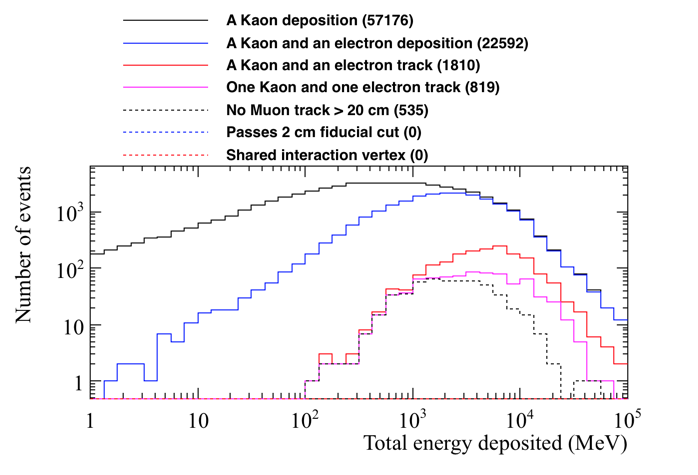
\includegraphics[width=0.8\textwidth]{CosmicBackground_EnergyDepCuts_Raw_2cmCut}
  \caption[The energy distribution of background events surviving the application of sequential cuts in the $n \rightarrow K^{+} + e^{-}$ channel]
          {The energy distribution of background events surviving the application of sequential cuts in the $n \rightarrow K^{+} + e^{-}$ channel. The total energy deposited in the detector is plotted on the $x$ axis.}
  \label{fig:NDK_CosmoBack_Raw}
\end{figure}

\begin{figure}[h!]
  \centering
  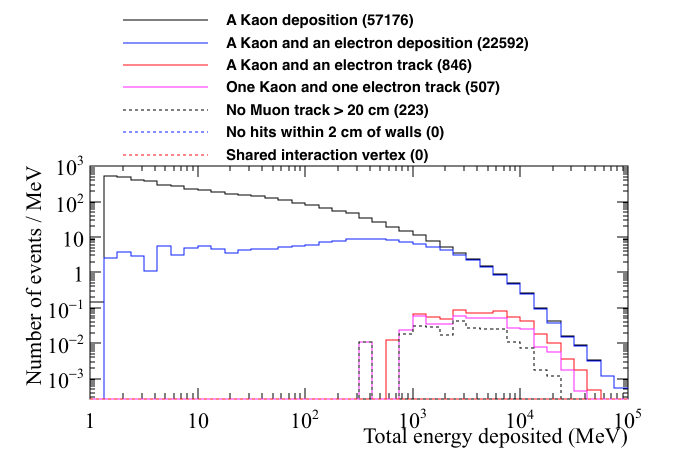
\includegraphics[width=0.8\textwidth]{CosmicBackground_EnergyDepCuts_Norm_2cmCut}
  \caption[The normalised energy distribution of background events surviving the application of sequential cuts in the $n \rightarrow K^{+} + e^{-}$ channel]
          {The normalised energy distribution of background events surviving the application of sequential cuts in the $n \rightarrow K^{+} + e^{-}$ channel. The total energy deposited in the detector is plotted on the $x$ axis. The normalised energy distribution has been found by dividing the number of events within a bin by the bin energy.}
  \label{fig:NDK_CosmoBack_Norm}
\end{figure}

From Figures~\ref{fig:NDK_CosmoBack_Raw} and~\ref{fig:NDK_CosmoBack_Norm}, it can be seen that there are no background events which could mimic a decay signature as there no events which survive the application of all cuts. This corresponds to a limit on the cosmogenic background to the $n \rightarrow K^{+} + e^{-}$ decay channel of XX$\times$10$^XX$. \\

It is interesting to observe the effect that relaxing some of the cuts has on the background rate. For example, the cuts after the presence of at least one kaon track, and at least one electrons shower, in the event have been confirmed, could be relaxed. This would allow for the effectiveness of each of the subsequent cuts to be observed. Initially, each of the four subsequent cuts are applied in isolation. The number of events surviving each of the cuts is shown in Table~\ref{tab:NDK_CosmoBack_EachCut}. \\

\begin{table}[h!]
  \caption[The number of events which could mimic a $n \rightarrow K^{+} + e^{-}$ decay, when cuts are applied in isolation]
          {The number of events which could mimic a $n \rightarrow K^{+} + e^{-}$ decay, when cuts are applied in isolation. Cuts are applied after it is found that the event contains at least one kaon track, and at least one electron shower. It is found that 1810 events have at least one kaon track, and at least one electron shower, this is shown in the top line of the table. The fiducial cut of 2 cm is seen to remove all of the events considered.}
  \centering
  \label{tab:NDK_CosmoBack_EachCut}
  \begin{tabular}{c c}
    \toprule
        {Cut that is applied}                                & {Num. events surviving cut} \\
        \midrule
        At least one kaon track, and electron shower         & 1810                                \\

        Only one kaon track, and only one electron shower    & 819                                 \\

        No muon track that is longer than 20 cm in length    & 1303                                \\

        No energy depositions within 2 cm of detector edge   & 0                                   \\

        The kaon and electron share a common vertex          & 137                                 \\
        \bottomrule
  \end{tabular}
\end{table}

The effectiveness of the fiducial cut is clearly apparent from Table~\ref{tab:NDK_CosmoBack_EachCut}, as it removes all 1810 events where there is both a kaon track and an electron shower. It is for this reason that the loss in fiducial volume that it causes is accepted. The requirement made on the proximity of the kaon track and electron shower is also seen to be very effective at removing background events. It is found that of the 819 events that have a single kaon track, and a single electron shower, in only 44 of them would the kaon and electron be considered to have a common vertex. When the additional constraint of there not being a muon with a track length of more than 20 cm present in the event is applied, only 14 events would survive the cuts. This shows that the only way to remove all potential background events is to apply the fiducial cut, or to make the some of the other criteria stricter, such as reducing the separation of the kaon track and the electron shower which constitutes a common vertex. \\

%********************************** % Fifth.Second Section  *************************************
\subsection{Signal events in the $n \rightarrow K^{+} + e^{-}$ decay channel} \label{sec:NDKSig}
It is important to confirm that the cuts developed to reject cosmic backgrounds, do not adversely affect the identification of nucleon decay events. For this reason, a sample of 10,000 neutron decay events in the DUNE far detector were generated using GENIE. Neutron decays are generated at random positions within the detector volume, and so it is possible that the decay occurs in the gaps between TPC volumes, as shown in Figure~\ref{fig:NDK_Sig_KEBigGap}, or near the edge of the detector, as is shown in Figure~\ref{fig:NDK_Sig_KENearEdge}. \\

\begin{figure}[h!]
  \centering
  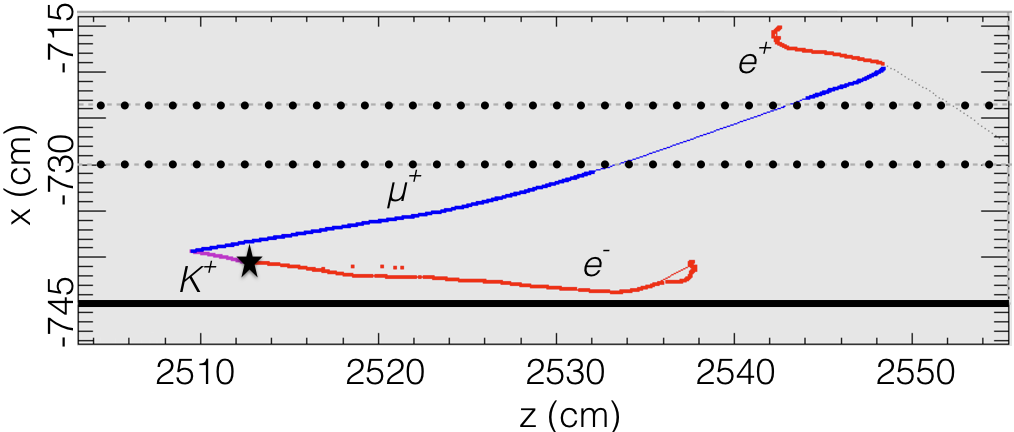
\includegraphics[width=0.8\textwidth]{KaonElecNearEdge}
  \caption[A simulated $n \rightarrow K^{+} + e^{-}$ decay which occurred near the edge of the detector volume]
          {A simulated $n \rightarrow K^{+} + e^{-}$ decay which occurred near the edge of the detector volume. The path of the kaon produced in the decay is shown as a purple line. The path of the muon, produced by the decay of the kaon, is shown as a blue line. The paths which the electrons in the event took are shown as red lines. The electron at the bottom of the figure is the electron produced in the neutron decay, whilst the one at the top of the figure, is produced by the decay of the muon. The thin coloured lines show track segments which were in uninstrumented parts of the detector, such as gaps between TPCs and APAs. The solid black line shows the edge of the detector. The dotted black lines show the edges of the TPCs, and the black star shows the location at which the decay occurred. It can be seen that though the event is contained within the detector it is very close to the edge of the detector due to the location at which the decay occurred.}
  \label{fig:NDK_Sig_KENearEdge}
\end{figure}

The analysis performed on the cosmogenic background was primarily designed to reject background events, whilst also attempting to not use cuts which would also affect signal efficiency. Therefore, it is hoped that the loss of signal events will be minimal. When running the analysis on the simulated signal events, the same definitions for tracks, showers, and the ancestry of particles are used, as well as the same cuts that were outlined in Section~\ref{sec:NDKCosmBk}. \\

The energy distribution of the signal events surviving the application of the sequential cuts is shown in Figure~\ref{fig:NDK_Sig_Raw}, this is the equivalent of Figure~\ref{fig:NDK_CosmoBack_Raw} for the cosmogenic background sample. The normalised energy distribution of signal events surviving the application of sequential cuts is shown in Figure~\ref{fig:NDK_Sig_Norm}, this is the equivalent of Figure~\ref{fig:NDK_CosmoBack_Norm} for the cosmogenic background sample. As before, the distribution of normalised energies is found by dividing the number of events by the bin energy. \\

\begin{figure}[h!]
  \centering
  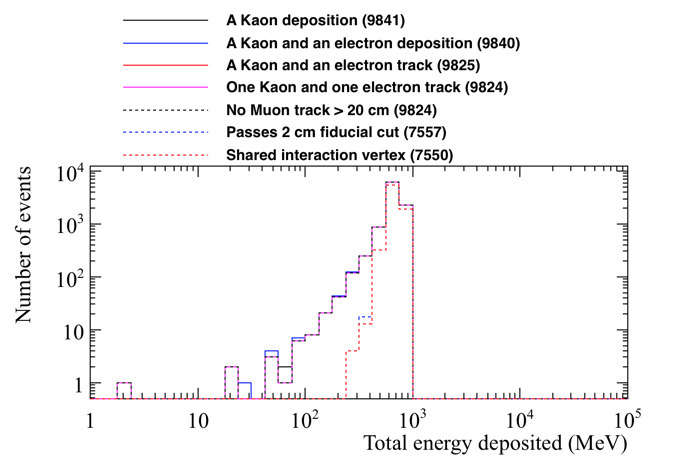
\includegraphics[width=0.8\textwidth]{NucleonDecay_EnergyDepCuts_Raw_2cmCut}
  \caption[The energy distribution of signal events surviving the application of sequential cuts in the $n \rightarrow K^{+} + e^{-}$ channel]
          {The energy distribution of signal events surviving the application of sequential cuts in the $n \rightarrow K^{+} + e^{-}$ channel. The total energy deposited in the detector is plotted on the $x$ axis.}
  \label{fig:NDK_Sig_Raw}
\end{figure}

\begin{figure}[h!]
  \centering
  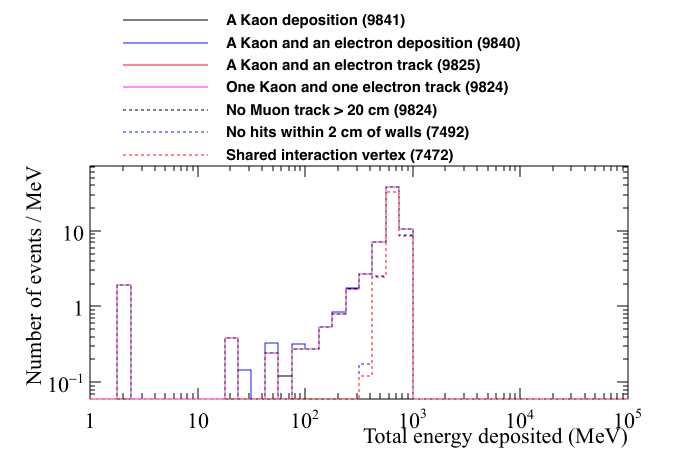
\includegraphics[width=0.8\textwidth]{NucleonDecay_EnergyDepCuts_Norm_2cmCut}
  \caption[The normalised energy distribution of signal events surviving the application of sequential cuts in the $n \rightarrow K^{+} + e^{-}$ channel]
          {The normalised energy distribution of signal events surviving the application of sequential cuts in the $n \rightarrow K^{+} + e^{-}$ channel. The total energy deposited in the detector is plotted on the $x$ axis. The normalised energy distribution has been found by dividing the number of events within a bin by the bin energy.}
  \label{fig:NDK_Sig_Norm}
\end{figure}

When comparing Figures~\ref{fig:NDK_Sig_Raw} and~\ref{fig:NDK_Sig_Norm} with Figures~\ref{fig:NDK_CosmoBack_Raw} and~\ref{fig:NDK_CosmoBack_Norm}, the most obvious difference is that when considering the nucleon decay events, the total energy deposited in the detector never exceeds 1 GeV, whilst in the cosmogenic background sample, the energy deposited in the detector frequently exceeds 1 GeV. This is something which one would expect, as the simulated neutrons decay at rest, and so have a total energy of less than 1 GeV, meaning that there cannot be more than 1 GeV deposited in the detector. This is in stark contrast to the cosmogenic background, where the primary muons being generated have a mean energy of 283 GeV, as shown in Table~\ref{tab:MUSUNflux}. This means that many events will deposit significant amounts of energy in the detector, even if the primary muon narrowly misses the detector volume. \\

The initial cuts, requiring that both a kaon track and an electron shower are observed in the decay, show that there are occasions when either the kaon, or the electron, do not deposit energy in the detector. This affects very few events, though an example of one such event is shown in Figure~\ref{fig:NDK_Sig_MissedKaon}, where it can be seen that the kaon decayed before entering the active volume, and so no track was found for it. It would be very difficult to identify this event as a signal event, as the presence of the kaon could only be inferred from the muon originating from the gap between the APAs, and the energy deposited by the kaon itself will not be reconstructed. Further compounding the identification of this event as a signal event, is the fact that the electron produced in the nucleon decay scatters back into the gap between the APAs. This means that a significant amount of the rest mass energy of the neutron would not be reconstructed. \\

\begin{figure}[h!]
  \centering
  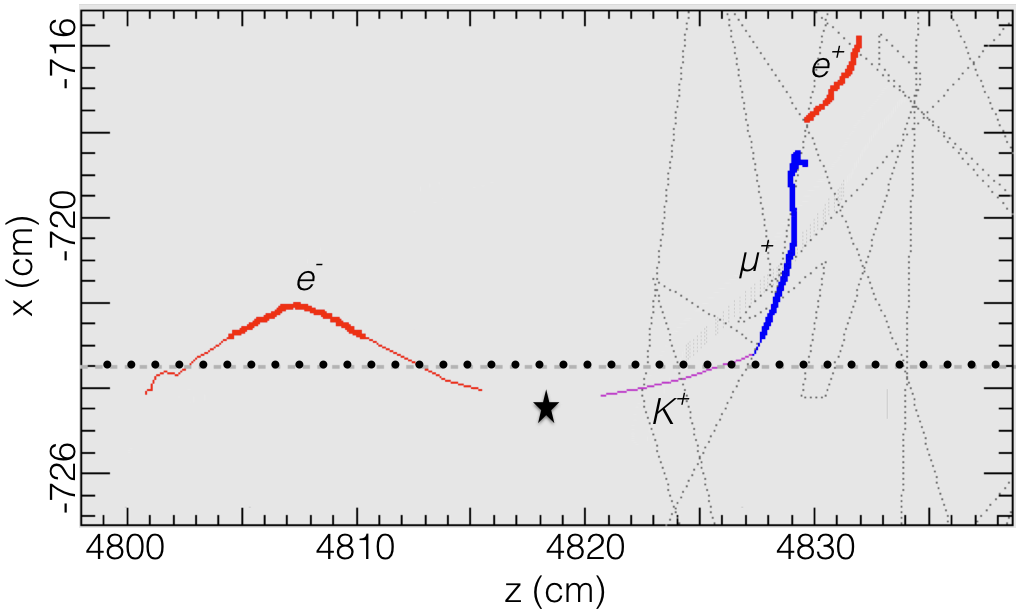
\includegraphics[width=0.8\textwidth]{MissedKaon}
  \caption[A simulated $n \rightarrow K^{+} + e^{-}$ decay where the kaon did not deposit any energy in the active volume]
          {A simulated $n \rightarrow K^{+} + e^{-}$ decay where the kaon did not deposit any energy in the active volume. The path of the kaon produced in the decay is shown as a purple line. The path of the muon, produced by the decay of the kaon, is shown as a blue line. The paths which the electrons in the event took are shown as red lines. The electron on the left of the figure is the electron produced in the neutron decay, whilst the one on the right of the figure, is produced by the decay of the muon. The thin coloured lines show track segments which were in uninstrumented parts of the detector, such as gaps between TPCs and APAs. The dotted black lines show the edges of the TPCs, and the black star shows the location at which the decay occurred. It can be seen that the kaon decayed before it entered the active volume of the detector, and so no track was found for it. A significant portion of the distance which the electron from the decay travelled was also outside the active volume of the detector.}
  \label{fig:NDK_Sig_MissedKaon}
\end{figure}

The number of events which are removed by the fiducial cut is concerning, as when it is considered in conjunction with other cuts it removes almost 23\% of events, this rises to almost 25\% of events when it is applied in isolation. This suggests that the cut is too strict. The reason for this is that protons and neutrons are emitted from the nucleus in many of the simulated decays. Whilst the protons produced will create relatively short tracks, which are connected to the decay vertex, the neutrons will travel large distances, and cause energy depositions which are far away from the decay vertex. The faint grey dashed lines, which can be seen in Figure~\ref{fig:NDK_Sig_MissedKaon}, show the spallation neutrons produced in the decay. None of the figures shown here contain spallation protons, but if they were present, they would be shown as additional purple lines originating from the decay vertex. It is predominantly the energy depositions from the spallation neutrons which are causing events to fail the ``no energy depositions within 2 cm of the detector edge'' cut. As a result it is likely that this cut needs to be relaxed, to instead be a cut on the amount of energy deposited within 2 cm of the detector edge. Figure~\ref{fig:NDK_EDepNearEdge} shows the amount of energy deposited within 2 cm, 5 cm, and 10 cm of the detector edges, for the simulated nucleon decay events (top), and the cosmogenic background events (bottom). \\ 

\begin{figure}[h!]
  \centering
  \begin{subfigure}{0.75\textwidth}
    \centering
    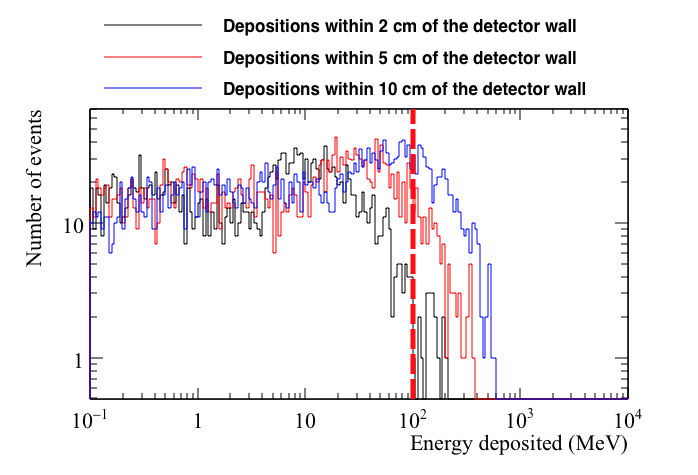
\includegraphics[width=\textwidth]{NucleonDecay_EDepNearEdges}
    \caption{The nucleon decay events.}
  \end{subfigure}
  % ========
  \begin{subfigure}{0.75\textwidth}
    \centering
    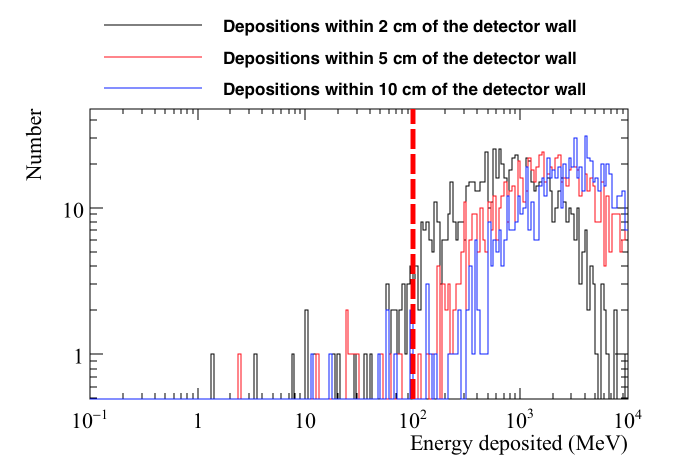
\includegraphics[width=\textwidth]{CosmicBackground_EDepNearEdges}
    \caption{The cosmogenic background events.}
  \end{subfigure}
  % ========
  \caption[The number of events, as a function of the energy deposited within 2 cm, 5 cm, and 10 cm of the detector edges.]
          {The number of events, as a function of the energy deposited within 2 cm, 5 cm, and 10 cm of the detector edges. Top shows the energies which were deposited for the simulated neutron decay events. Bottom shows the energies which were deposited in the simulated cosmogenic background events. The histograms are filled after the cut requiring that there is at least one kaon track, and at least one electron shower in the event, is applied. As such, the histograms are filled with 9824 and 1810 events for the top and bottom histograms respectively. The dashed red line shows a preliminary cut on the energy deposited of 100 MeV.}
  \label{fig:NDK_EDepNearEdge}
\end{figure}

As can be seen from Figure~\ref{fig:NDK_EDepNearEdge}, the amount of energy deposited near the detector edges is very different in the nucleon decay, and cosmogenic background events. As such, they can be relatively cleanly separated. A very conservative cut, designed to preserve as many of the simulated signal events as possible, which demands that there be no more than 100 MeV of energy deposited within 2 cm of the detector edge is used. Requiring that there be no more 100 MeV of energy deposited within 2 cm of the detector edges, removes only 19 of the 9824 signal events, whilst only 171 out of the 535 cosmic background events meet this requirement. Whilst this does mean that the fiducial cut no longer removes every event in the cosmic background sample, it does not cause the huge loss of signal events which was seen when the hard cut, of no energy depositions within 2 cm of the detector edge, was used. It is also important to remember that the requirement that the kaon track and the electron shower share a common vertex, as well as cuts on the energy deposition profiles, will still be applied to these 171 background events. For example, only 2 of the 171 events satisfy the requirement that the kaon track and the electron shower share a common vertex. It will be seen in Section~\ref{sec:NDKEnCosmBk}, that the 2 events sharing a common vertex do not satisfy the energy distributions expected from a nucleon decay event. \\

The definition used to decide if the start of the kaon track, and the start of the electron shower, share a common vertex seems to be a reasonable requirement, as almost all of the signal events satisfy this definition. The distance between the start of the kaon track, and the start of the electron shower is shown in Figure~\ref{fig:NDK_Sig_KEDist}. It can be seen that the separation between the two particles is very small (<0.1 cm) in most events. However, there are some events where the separations are very large (>10 cm). As discussed earlier, the decays in these events occur in the gaps between TPCs, such as that shown in Figure~\ref{fig:NDK_Sig_KEBigGap}. When the requirement that the kaon track and the electron shower have a PoCA of less than 2 cm is then applied to these events, most of them are then seen to have a common interaction vertex. For example, this is found to be the case for the event shown in Figure~\ref{fig:NDK_Sig_KEBigGap}. However, in some events the kaon track, and the electron shower, are still not found to have a common interaction vertex. Hand scanning of these events shows that in these events, the particles undergo scattering before entering the active volume, and so by the time that the energy depositions are collected, their trajectories are no longer closely aligned. This causes the calculated values of PoCA to be larger than 2 cm, and so they do meet the requirement that their trajectories are closely aligned. \\

\begin{figure}[h!]
  \centering
  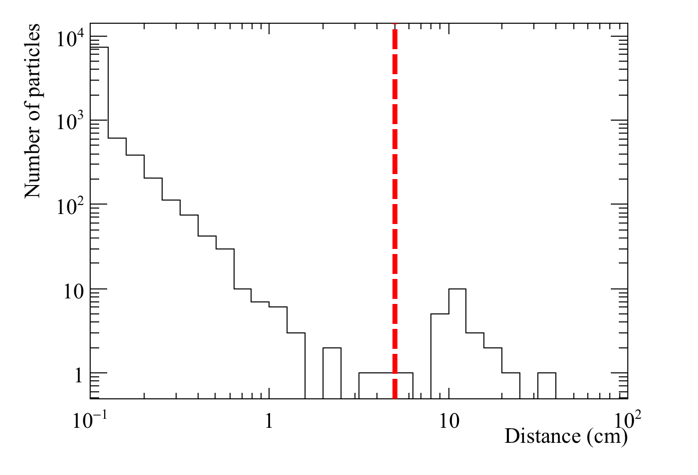
\includegraphics[width=0.8\textwidth]{NucleonDecay_KaonElecSep}
  \caption[The separation of the kaon and the electron produced in the $n \rightarrow K^{+} + e^{-}$ decay channel]
          {The separation of the kaon and the electron produced in the $n \rightarrow K^{+} + e^{-}$ decay channel. The dashed red line, drawn at a separation of 5 cm, shows the maximum possible separation a kaon and an electron could have, and still be considered to have a common vertex.}
  \label{fig:NDK_Sig_KEDist}
\end{figure}

The normalised energy distributions of simulated decay events, and simulated cosmogenic background events, after the fiducial cut is changed to be a limit of 100 MeV of energy deposited within 2 cm of the detector edge, is shown in Figure~\ref{fig:NDK_FidCut_EnLim}. As before, the distribution of normalised energies is found by dividing the number of events by the bin energy. \\

\begin{figure}[h!]
  \centering
  \begin{subfigure}{0.8\textwidth}
    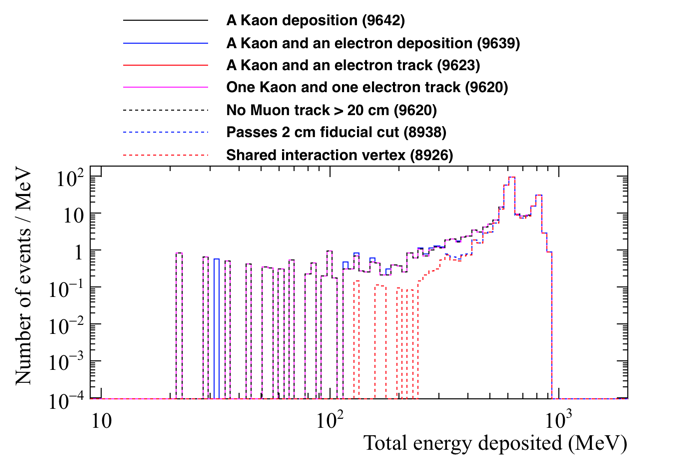
\includegraphics[width=\textwidth]{NucleonDecay_EnergyDepCuts_Norm}
    \caption{The normalised energy distribution of signal events.}
    \label{fig:NDK_FidCut_EnLim_Sig}
  \end{subfigure}
  % ========
  \begin{subfigure}{0.8\textwidth}
    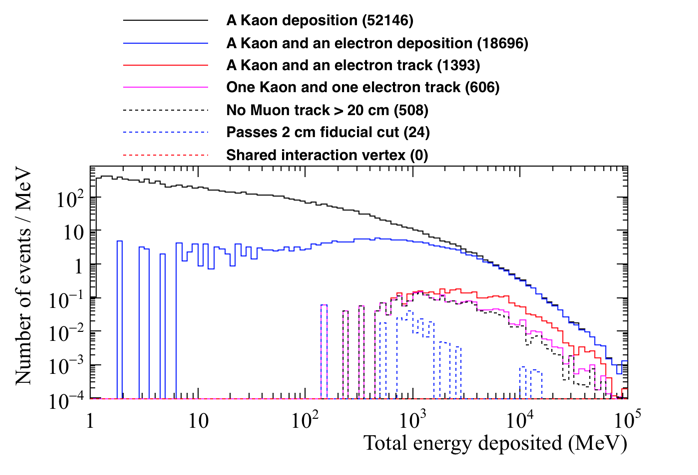
\includegraphics[width=\textwidth]{CosmicBackground_EnergyDepCuts_Norm}
    \caption{The normalised energy distribution of cosmic background events.}
    \label{fig:NDK_FidCut_EnLim_Cosmo}
  \end{subfigure}
  \caption[The normalised energy distribution of signal events, and cosmic background events, surviving the application of sequential cuts, after the fiducial cut is modified]
          {The normalised energy distribution of signal events, and cosmic background events, surviving the application of sequential cuts, after the fiducial cut is modified. The total energy deposited in the detector is plotted on the $x$ axis. The normalised energy distribution has been found by dividing the number of events within a bin by the bin energy.}
  \label{fig:NDK_FidCut_EnLim}
\end{figure}

The number of signal events which are removed by the cuts can be seen to be much more reasonable after the fiducial cut is modified, as less than 2.5\% of signal events are removed as cuts are applied. It is seen that in many of the simulated decay events which fail the cuts, at least one of the kaon, or the electron, are not contained in the detector. This means that, either no depositions are found for the particle, or it deposits significant amounts of energy as it leaves the detector. \\

It can be seen that though 2 of the cosmic background events pass the application of all cuts, the total energy deposited in the detector is not less than 1 GeV in either of these events. This means that the total energy deposited in the detector is more than the rest mass of a neutron, and so the event is not consistent with being from the decay of a neutron at rest. However, it is still prudent to determine the expected energy deposition distribution for the signal events, in order to ensure that a clean separation can be observed between the signal, and background events.  \\

%********************************** % Fifth.Second Section  *************************************
\subsection{Energy constraints on the cosmogenic background to the $n \rightarrow K^{+} + e^{-}$ decay channel} \label{sec:NDKEnCosmBk}
As outlined in Section~\ref{sec:NDKCosmBk}, it is possible to exclude background events from signal events, using the distribution of how energy is deposited in the detector. The energy criteria which were previously outlined were;
\begin{itemize}
\item The energy directly deposited by the kaon.
\item The energy deposited by the kaon decay products.
\item The energy directly deposited by the electron.
\item The energy deposited near the shared kaon and electron vertex.
\item The energy deposited in the detector which does not fit any of the above criteria.
\end{itemize}
Following the earlier discussions in Section~\ref{sec:DUNENDK}, it should be clear that the energy directly deposited by the kaon corresponds to the sum of all energy depositions, which are due to the kaon or its interaction products. Equivalently, the energy directly deposited by the electron, corresponds to the sum of all energy depositions which are due to the electron as it showers, and any particles created as a result of the shower. The energy deposited by the kaon decay products would include all depositions by the muon and subsequent electron, in the case that the kaon decayed via $K^{+} \rightarrow \mu^{+} + \nu_{\mu}$, and then the muon decayed via $\mu^{+} \rightarrow e^{+} + \nu_{e} + \nu_{\mu}$. The energy deposited near the shared kaon and electron vertex, would primarily consist of energy depositions due to spallation products. These depositions would largely be due to protons, though may also include some depositions due to neutrons too, if they deposited energy near the interaction vertex. Any depositions within 5 cm of either, the start of the kaon track, or the start of the electron shower, are considered 'near' to the interaction vertex. It is necessary to consider the energy depositions which are close to the start of both particles, because, as shown in Figure~\ref{fig:NDK_Sig_KEBigGap}, occasionally the particles are separated by the APA gaps. When energy depositions are within 5 cm of both, the start of the kaon track, and the electron shower, they are only considered to be near to the start of the kaon track. This is done so as to avoid 'double counting' these energy depositions. As can be seen from Figure~\ref{fig:NDK_Sig_KEDist}, the separation between the start of the kaon track, and the start of the electron shower, is normally very small. This means that the sum of the 'near' energy depositions, can be considered to be the energy depositions 'near' the common vertex between the kaon track and the electron shower. The final criteria, of any depositions which do not fit the above description, would largely consist of energy depositions due to the spallation neutrons in the decay sample. However, in the cosmic background sample, this would include all depositions by muons, pions, and any other particles in the detector, which are not associated with either the kaon or the electron. In later discussions these depositions are generally labelled as 'other' energy depositions. \\

In presenting the separation of simulated cosmic background events, and simulated neutron decay events, the important distributions to consider are as follows:
\begin{itemize}
\item The energy directly deposited by the kaon, against the energy directly deposited by the electron. This is shown in Figure~\ref{fig:NDK_Kaon_Elec_EDist}.
\item The energy directly deposited by the kaon, plus the energy directly deposited by the electron, against the energy deposited near the shared kaon and electron vertex. This is shown in Figure~\ref{fig:NDK_KaonElec_Near_EDist}.
\item The energy deposited by the kaon, including decay products, against the energy deposited in the detector which does not fit any of the other criteria. This is shown in Figure~\ref{fig:NDK_AllKaon_Other_EDist}.
\item The energy deposited by the kaon, including decay products, plus the energy directly deposited by the electron, plus the energy deposited near the shared kaon and electron vertex, against the energy deposited in the detector which does not fit any of the other criteria. This is shown in Figure~\ref{fig:NDK_AllEDep_Other_EDist}.
\end{itemize}
Each of these figures will be discussed in turn below. \\

When looking at the figures presented, the events which pass all cuts in the simulated decay sample have been plotted with smaller markers. This is to allow the events which fail the cuts to be visible. The markers have also been plotted so as to have the earlier cuts in the foreground in the nucleon decay sample, and the later cuts to be in the foreground in the cosmic background sample. This is done so as to prevent the events which fail (pass) the cuts, from being overwhelmed by the more numerous events which pass (fail) the cuts, in the simulated nucleon decay (cosmic background) sample. \\

Additionally, in the figures outlined above, there is a box in the lower left corner of the plots, produced by dashed grey lines. This constitutes the expected energy region where a signal event would lie on the graph, and has been drawn so as to contain as many of the simulated signal events as possible. The expected energy regions are propagated down to 0 MeV on both the $x$ and $y$ axis of all figures, and so it is possible for points not drawn here to pass the applied cuts. This is because it is possible for signal events to have either no energy identified as 'near' the common interaction vertex, such as the event shown in Figure~\ref{fig:NDK_Sig_KEBigGap}. It is also possible for there to be no energy deposited in the detector which would be classed as 'other' energy depositions. \\

% ========== Kaon vs Elec
\begin{figure}[h!]
  \centering
  \begin{subfigure}{0.8\textwidth}
    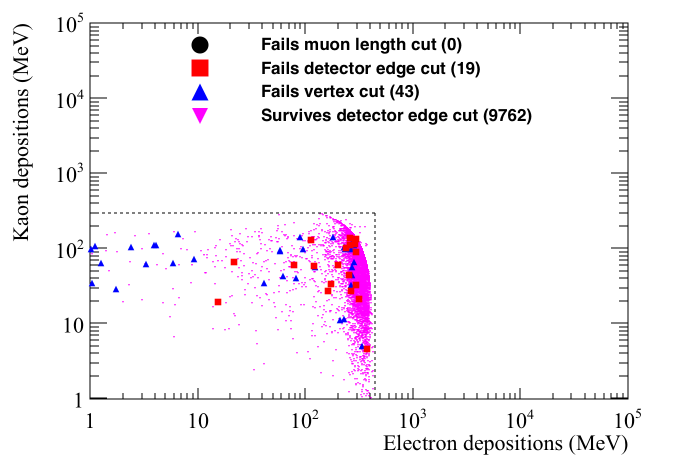
\includegraphics[width=\textwidth]{NucleonDecay_Kaon_vs_Elec_Can}
    \caption{The energy distribution of signal events.}
    \label{fig:NDK_Kaon_Elec_EDist_Sig}
  \end{subfigure}
  % ========
  \begin{subfigure}{0.8\textwidth}
    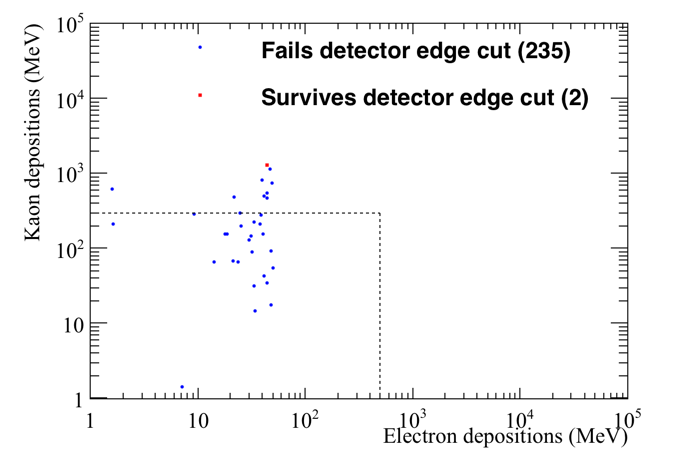
\includegraphics[width=\textwidth]{CosmicBackground_Kaon_vs_Elec_Can}
    \caption{The energy distribution of cosmic background events.}
    \label{fig:NDK_Kaon_Elec_EDist_Cosmo}
  \end{subfigure}
  \caption[The energy directly deposited by kaons, as a function of the energy directly deposited by electrons, in the simulated nucleon decay, and cosmic background samples]
          {The energy directly deposited by kaons, as a function of the energy directly deposited by electrons, in the simulated nucleon decay, and cosmic background samples. The events failing the application of the muon length (black circle), fiducial (red box) and vertex (blue triangle) cuts, as well as the events passing all cuts (pink triangle) are shown.}
  \label{fig:NDK_Kaon_Elec_EDist}
\end{figure}

% ========== Kaon + Elec vs Near
\begin{figure}[h!]
  \centering
  \begin{subfigure}{0.8\textwidth}
    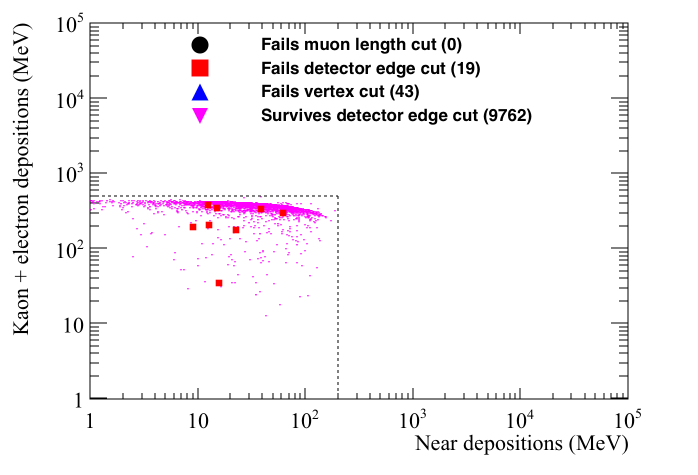
\includegraphics[width=\textwidth]{NucleonDecay_KaonElec_vs_Near_Can}
    \caption{The energy distribution of signal events.}
    \label{fig:NDK_KaonElec_Near_EDist_Sig}
  \end{subfigure}
  % ========
  \begin{subfigure}{0.8\textwidth}
    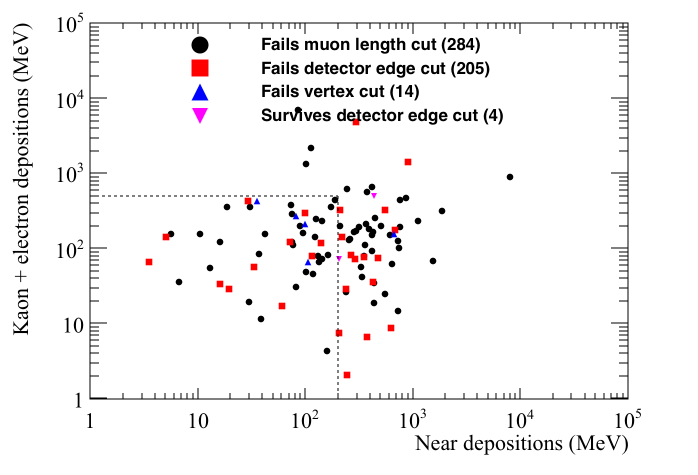
\includegraphics[width=\textwidth]{CosmicBackground_KaonElec_vs_Near_Can}
    \caption{The energy distribution of cosmic background events.}
    \label{fig:NDK_KaonElec_Near_EDist_Cosmo}
  \end{subfigure}
  \caption[The energy directly deposited by kaons, plus the energy directly deposited by electrons, as a function of the energy deposited near the kaon and electron vertex, in the simulated nucleon decay, and cosmic background samples]
          {The energy directly deposited by kaons, plus the energy directly deposited by electrons, as a function of the energy deposited near the kaon and electron vertex, in the simulated nucleon decay, and cosmic background samples. The events failing the application of the muon length (black circle), fiducial (red box) and vertex (blue triangle) cuts, as well as the events passing all cuts (pink triangle) are shown.}
  \label{fig:NDK_KaonElec_Near_EDist}
\end{figure}

% ========== Kaon + Kaon Decay vs Other
\begin{figure}[h!]
  \centering
  \begin{subfigure}{0.8\textwidth}
    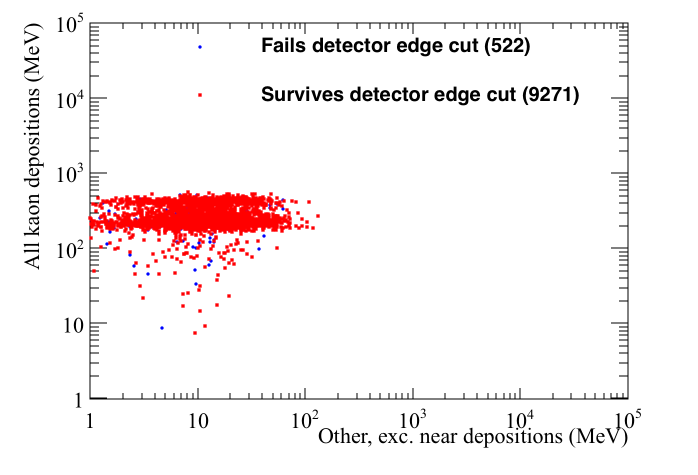
\includegraphics[width=\textwidth]{NucleonDecay_AllKaon_vs_Other_Can}
    \caption{The energy distribution of signal events.}
    \label{fig:NDK_AllKaon_Other_EDist_Sig}
  \end{subfigure}
  % ========
  \begin{subfigure}{0.8\textwidth}
    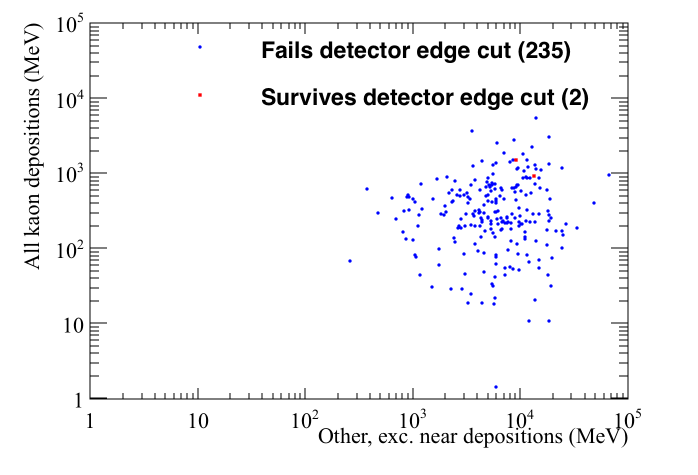
\includegraphics[width=\textwidth]{CosmicBackground_AllKaon_vs_Other_Can}
    \caption{The energy distribution of cosmic background events.}
    \label{fig:NDK_AllKaon_Other_EDist_Cosmo}
  \end{subfigure}
  \caption[The energy directly deposited by kaons, plus the energy deposited by the kaon decay products, as a function of the energy depositions which do not fit any of the other criteria, in the simulated nucleon decay, and cosmic background samples]
          {The energy directly deposited by kaons, plus the energy deposited by the kaon decay products, as a function of the energy depositions which do not fit any of the other criteria, in the simulated nucleon decay, and cosmic background samples. The events failing the application of the muon length (black circle), fiducial (red box) and vertex (blue triangle) cuts, as well as the events passing all cuts (pink triangle) are shown.}
  \label{fig:NDK_AllKaon_Other_EDist}
\end{figure}

% ========== Kaon + Kaon Decay + Elec + Near vs Other
\begin{figure}[h!]
  \centering
  \begin{subfigure}{0.8\textwidth}
    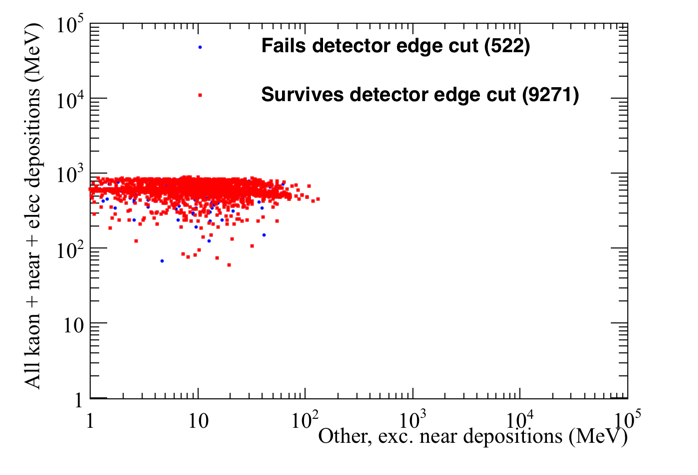
\includegraphics[width=\textwidth]{NucleonDecay_AllKaonNearElec_vs_Other_Can}
    \caption{The energy distribution of signal events.}
    \label{fig:NDK_AllEDep_Other_EDist_Sig}
  \end{subfigure}
  % ========
  \begin{subfigure}{0.8\textwidth}
    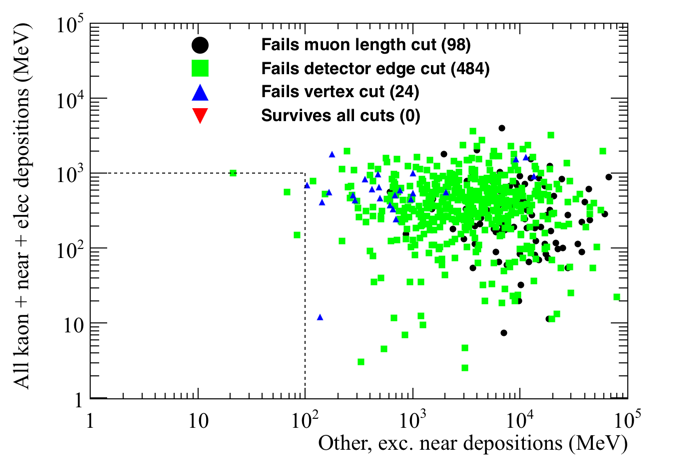
\includegraphics[width=\textwidth]{CosmicBackground_AllKaonNearElec_vs_Other_Can}
    \caption{The energy distribution of cosmic background events.}
    \label{fig:NDK_AllEDep_Other_EDist_Cosmo}
  \end{subfigure}
  \caption[The energy directly deposited by kaons, plus the energy deposited by the kaon decay products, plus the energy directly deposited by electrons, plus the energy deposited near the kaon and electron vertex, as a function of the energy depositions which do not fit any of the other criteria, in the simulated nucleon decay, and cosmic background samples]
          {The energy directly deposited by kaons, plus the energy deposited by the kaon decay products, plus the energy directly deposited by electrons, plus the energy deposited near the kaon and electron vertex, as a function of the energy depositions which do not fit any of the other criteria, in the simulated nucleon decay, and cosmic background samples. The events failing the application of the muon length (black circle), fiducial (red box) and vertex (blue triangle) cuts, as well as the events passing all cuts (pink triangle) are shown.}
  \label{fig:NDK_AllEDep_Other_EDist}
\end{figure}

% ========== Kaon vs Elec
From Figure~\ref{fig:NDK_Kaon_Elec_EDist}, it can be seen that the electron energy distribution in the cosmic background sample, is very different from the one seen in the simulated neutron decay sample. This is shown by the energies deposited by electrons in the nucleon decay sample being tightly concentrated between $\sim$200 and $\sim$400 MeV, whilst in the cosmic background sample, the energy deposited by the electron is almost always less than $\sim$50 MeV. Many of the electrons in the cosmic background sample deposit less than 1 MeV of energy in the detector, and so are not shown in Figure~\ref{fig:NDK_Kaon_Elec_EDist_Cosmo}. This is why the events where the kaon and electron share a common vertex are not shown in the cosmic background sample, as the electrons in these events deposit less than 1 MeV of energy in the detector. Realistically, these electrons are unlikely to be reconstructed due to their extremely low energies. From Figure~\ref{fig:NDK_Kaon_Elec_EDist_Sig}, it can be seen that some of the electrons produced in the nucleon decay events also deposit very little energy in the detector, though these events generally fail either the fiducial cut, or the vertex cut. An explanation as to why these events fail the cuts was presented in Section~\ref{sec:NDKSig}, when considering Figure~\ref{fig:NDK_Sig_MissedKaon}. \\

% ========== Kaon + Elec vs Near
From Figure~\ref{fig:NDK_KaonElec_Near_EDist}, it can be seen that for the simulated nucleon decay events, as the energy deposited near the kaon and electron vertex increases, the sum of the energy deposited by the kaon and electron decreases. This is reasonable, because, when the spallation protons and neutrons have more energy, the kaon and electron will have less energy. The decrease in the energy deposited by the kaon and the electron, is roughly consistent with the increase in the amount of energy which is deposited near their shared vertex. This means that the sum of the three energies is generally around 450 MeV. This is largely inconsistent with the simulated cosmic background events, where many events have no energy deposited near the shared vertex of the kaon and electron. However, the lack of energy deposited near the shared kaon and electron vertex cannot be used to discriminate against cosmogenic background events, as this is also observed in many simulated nucleon decay events. What can be used to separate cosmic background events from nucleon decay events though, is the sum of the three energy criteria, as it can be seen that this would rarely be around 450 MeV in the cosmic background sample. \\

% ========== Kaon + Kaon Decay vs Other
Figure~\ref{fig:NDK_AllKaon_Other_EDist}, shows that the sum of all energy deposits attributed to the kaon, against the sum of all energy depositions which are considered to be 'other' energy depositions, is very different in the two samples. The total energy deposited in the detector which is attributed to the kaon, is found by combining the energy directly deposited by the kaon, with the energy deposited by the kaon decay products. The difference seen in the cosmogenic and signal events, is primarily due to the large amount of 'other' energy depositions which are seen in the cosmogenic background sample. This is expected, as in cosmogenic induced events, many particles may enter the detector, and they will cause energy depositions which are not connected to the kaon track, the electron shower, or their common vertex, should one exist. This gives the most powerful mechanism for the discrimination between signal and background events, as in many background events the 'other' energy deposited in the detector will be very large, and will cause the total energy deposited in the detector to be more than the rest mass of a neutron. Also, the 'other' energy deposited by background events in the detector, will likely be concentrated in track or shower like structures. This is in contrast to signal events, where the 'other' energy depositions are likely to be isolated depositions due to the spallation neutrons interacting in the detector. Classifying the structure of the 'other' energy depositions is not performed here, though it could be included should any cosmic events appear to mimic a signal event. However, given the clear separation in the amount of 'other' energy deposited in the detector, it is not currently required. \\

A striking feature of Figure~\ref{fig:NDK_AllKaon_Other_EDist_Sig}, is the banded structure of the total energy deposited in the detector which can be attributed to the kaon. This banded structure is due to the amount of energy from the kaon decay which is not reconstructed. The relative strengths of these structural features is due to the various probabilities of the kaon decay modes. Some of the more common decay modes are shown in Table~\ref{tab:NDK_KaonDecayRat}, along with their probabilities. The amount of energy which is reconstructed from the particles produced by the decay of the kaon is shown in Figure~\ref{fig:NDK_KaonDecayEn}. \\

\begin{table}[h!]
  \caption[The most common decay modes of charged kaons, and their probabilities]
          {The most common decay modes of charged kaons, and their probabilities~\citep{PDGReview}. The decay modes shown are with reference to $K^{+}$, though the decays of $K^{-}$ are the charge conjugations of these decays.}
  \centering
  \label{tab:NDK_KaonDecayRat}
  \begin{tabular}{c c}
    \toprule
        {Decay mode}                                      & {Measured probability (\%)} \\
        \midrule
        $K^{+} \rightarrow \mu^{+} + \nu_{\mu}$           & 63.56 $\pm$ 0.11 \\

        $K^{+} \rightarrow \pi^{+} + \pi^{0}$             & 20.67 $\pm$ 0.08 \\

        $K^{+} \rightarrow \pi^{+} + \pi^{+} + \pi^{-}$   & 5.583 $\pm$ 0.024 \\

        $K^{+} \rightarrow \pi^{0} + e^{+} + \nu_{e}$     & 5.07 $\pm$ 0.04 \\

        $K^{+} \rightarrow \pi^{0} + \mu^{+} + \nu_{\mu}$ & 3.352 $\pm$ 0.033 \\

        $K^{+} \rightarrow \pi^{+} + \pi^{0} + \pi^{0}$   & 1.760 $\pm$ 0.023 \\
        \bottomrule
  \end{tabular}
\end{table}

\begin{figure}[h!]
  \centering
  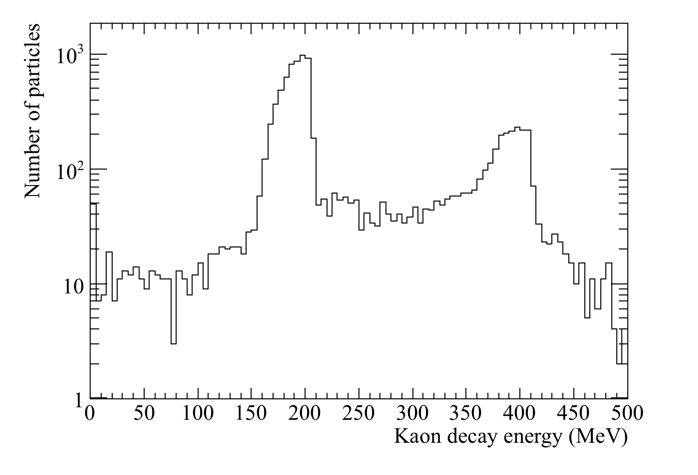
\includegraphics[width=0.8\textwidth]{NucleonDecay_KaonDecayEnergy}
  \caption[The number of events, as a function of the energy deposited by the kaon decay products.]
          {The number of events, as a function of the energy deposited by the kaon decay products. The energies deposited due to the $K^{+} \rightarrow \mu^{+} + \nu_{\mu}$ and $K^{+} \rightarrow \pi^{+} + \pi^{0}$ decay channels, can be seen in the peaks at roughly 200 MeV, and 400 MeV respectively. The underlying continuous distribution of deposited is caused by the 3-body decays shown in Table~\ref{tab:NDK_KaonDecayRat}.}
  \label{fig:NDK_KaonDecayEn}
\end{figure}

As can be seen in Table~\ref{tab:NDK_KaonDecayRat}, the most common decay mode for the kaon involves the production of a $\nu_{\mu}$, which will likely leave the detector without interacting. This will mean that a significant proportion of the kaon rest mass energy will not be reconstructed, as the kaon is assumed to decay at rest. It is for this reason that the most likely amount of energy deposited by the kaon decay products is around 200 MeV. The second most likely decay mode is also a 2-body decay, and one would expect that the energies from both the $\pi^{+}$ and $\pi^{0}$ would be reconstructed. Evidently some energy is either missed in the APAs gaps, or escapes the detector, as the second peak at 400 MeV, is less than the rest mass of the kaon. This missing energy is likely due to the energy associated with the decay of the $\pi^0$, as when it decays it is likely to produce two EM showers which may escape the detector, or deposit significant amounts of energy in the APA gaps. Neutrinos are also present in many of the other decay modes, and so will also have large amounts of missing energies, whilst the 3-body decay modes will produce particles which have a continuous distribution of energies. These decay modes, along with the missing, and lost energies, in the two most probable decay modes, cause the energy deposited by the kaon decay products to be a continuous distribution, with two large peaks at roughly 200 MeV and 400 MeV. The energy energy deposited by the kaon decay products in the cosmogenic background sample may not follow this energy profile, as it is likely that the kaon will not decay at rest. \\

% ========== Kaon + Kaon Decay + Elec + Near vs Other
Finally, Figure~\ref{fig:NDK_AllEDep_Other_EDist} shows the total energy attributed to both the kaon and to the electron, plus any energy deposited near their shared interaction vertex, against any 'other' energy depositions. As the total energy attributed to the kaon is plotted, this includes the energy deposited by the kaon decay products, as was the case in Figure~\ref{fig:NDK_AllKaon_Other_EDist}. As was seen in Figure~\ref{fig:NDK_AllKaon_Other_EDist}, there is a clear separation between the simulated signal events, and the cosmic background events. This is again due to the large amount of 'other' energy depositions observed in the background sample. It is interesting to compare Figures~\ref{fig:NDK_AllKaon_Other_EDist_Cosmo} and~\ref{fig:NDK_AllEDep_Other_EDist_Cosmo}, as they are very similar. This is to be expected from Figure~\ref{fig:NDK_Kaon_Elec_EDist_Cosmo}, where it was seen that the energy deposited by the electron was rarely more than 10 MeV, and only in one event was it more than 100 MeV. This was in stark contrast to Figure~\ref{fig:NDK_Kaon_Elec_EDist_Sig}, where the energy deposited in almost all of the electron showers was more than 100 MeV. It is for this reason that whilst there is a large difference in Figure~\ref{fig:NDK_AllKaon_Other_EDist_Sig} and~\ref{fig:NDK_AllEDep_Other_EDist_Sig}, due to addition of the significant amount of energy deposited by the electron showers, there is relatively little difference between Figures~\ref{fig:NDK_AllKaon_Other_EDist_Cosmo} and~\ref{fig:NDK_AllEDep_Other_EDist_Cosmo}. The change, or lack thereof, of the energy plotted between Figures~\ref{fig:NDK_AllKaon_Other_EDist} and~\ref{fig:NDK_AllEDep_Other_EDist}, thus provides another powerful metric by which to discriminate signal events, from background events. \\

A significant difference between Figures~~\ref{fig:NDK_AllKaon_Other_EDist_Sig} and~\ref{fig:NDK_AllEDep_Other_EDist_Sig}, is the relatively narrow band of energies plotted on the $y$ axis of Figure~\ref{fig:NDK_AllEDep_Other_EDist_Sig}, when compared to Figure~\ref{fig:NDK_AllKaon_Other_EDist_Sig}. This is because of the relationship between the energy deposited by the kaon, the energy deposited by the electron shower, and the energy deposited near their shared interaction vertex. This was seen in Figure~\ref{fig:NDK_KaonElec_Near_EDist_Sig}, where the sum of the three energies was roughly 450 MeV. This means that for events where the kaon deposited relatively little energy, shown by the population of events at low total kaon energies in Figure~\ref{fig:NDK_AllKaon_Other_EDist_Sig}, the energy deposited by the electron shower, plus the energy deposited near the shared interaction vertex, will be large. \\

Following the application of all energy cuts, as outlined by the grey dashed boxes in Figures~\ref{fig:NDK_Kaon_Elec_EDist},~\ref{fig:NDK_KaonElec_Near_EDist},~\ref{fig:NDK_AllKaon_Other_EDist}, and~\ref{fig:NDK_AllEDep_Other_EDist}, only 17 of the 9762 simulated signal events, which passed all subsequent cuts, are removed. It is found that none of the events survive the application of all cuts. If only the energy cuts, and the requirement that there be at least one kaon track, and at least one electron shower in the event, are applied, it is found that only 12 background candidates would survive the application of cuts. None of these events present serious contenders for signal events though, as all of events fail the vertex cut, and many have electrons which have very little energy (< 10 MeV), and large energy depositions near the edge of the detector. \\

Many of the signal events which are removed by the energy cuts have large amounts of 'other' energy depositions, though they would no longer be removed if the limit on 'other' depositions were raised to 200 MeV. Though increasing the cut on 'other' energy depositions to 200 MeV would still result in all background events being removed, it would mean that the limit was much closer to the regions of 'other' energy depositions which are populated in Figures~\ref{fig:NDK_AllKaon_Other_EDist}, and~\ref{fig:NDK_AllEDep_Other_EDist}. As a result if a candidate event were to have between 100 and 200 MeV of energy depositions considered to be 'other' energy depositions, its energy distributions would have to be carefully checked in order to verify that it is definitively not due to a background event. It is envisioned that the process by which this would be done, would be to consider how the 'other' energy deposits are distributed in the detector, because, as discussed earlier, in a signal event it is likely that they would be isolated depositions, whereas in a background event, there would likely be 'track-like' objects, which are disconnected from the kaon and electron vertex. \\

Therefore, the result of a preliminary study on the background rejection for the $n \rightarrow K^{+} + e^{-}$ decay channel, is that one would expect no cosmogenically induced background events in a single 10 kt module, over the course of XXX years of detector live time. In the absence of any candidate events, this would correspond to a partial lifetime of the neutron in the $n \rightarrow K^{+} + e^{-}$ decay channel of XXX $\times$ 10$^{-XX}$ years. \\

It is also found that using the cuts outlined above, only 2.55\% of signal events would not be identified as being from nucleon decay events. However, it would be difficult to identify many of the events considered here as nucleon decay events. This is because, in many events at least one of the kaon, or electron, leaves the detector. This would mean that accurate particle identification, and the correct calculation of initial kinetic energy, would be very difficult. Therefore, one could argue that the figure of 97.45\% nucleon decays being able to be identified as signal events is incorrect. This is because in only 9,216 of the 10,000 simulated decay events, are both the kaon, and the electron, contained in the detector. When only these 9,216 events are considered, it is found that 9,177 events survive the application of all cuts. This represents a signal efficiency of 99.58\%. It is found that the events which fail cuts either occur near the edge of the detector, as in Figure~\ref{fig:NDK_EDepNearEdge}, or scatter whilst outside of the active volume of the detector, as presented when discussing Figure~\ref{fig:NDK_Sig_KEBigGap}. As such, one could argue that the signal efficiency, using the cuts presented here is as high as 99.58\%. However, given the lack of signal mimicking background events observed in this study, it may be possible to identify many of the signal events where the kaon and/or electron are not contained in the detector, given the rest of the event topology. \\

%********************************** % Fifth.Third Section  *************************************
\subsection{Future improvements to nucleon decay studies and conclusions} \label{sec:NDKImprov}
Thus far, nucleon decay studies have only been performed on Monte Carlo truth information, and so have not used reconstructed objects. The extension of the analyses to include work on tracks is an important next step, as then the full analysis, which would be applied on real data, can be tested. Preliminary studies have begun on hit reconstruction, and involve running a filter on the muons used in the earlier analyses. This is because the number of events which are saved to disk would be prohibitive to running the full reconstruction process. As such, only events which meet the following criteria will be reconstructed~\citep{CosmoJanCollabMeeting};
\begin{itemize}
\item A minimum of 10 MeV deposited in the detector volume.
\item A maximum of 3,000 MeV deposited in the detector volume.
\item A maximum of 5 MeV deposited within 10 cm of the detector edge.
\end{itemize}
These criteria are designed to be broad enough that the full range of nucleon decay modes can be studied, including di-nucleon decay modes. This is why the maximum deposited energy greatly exceeds the rest mass of a single nucleon. This also accounts for the fact that during reconstruction some energy depositions may not be reconstructed, so even though the total energy deposited in the detector is 3 GeV, the total reconstructed energy may be less. \\

Upon performing reconstruction, and hence energy and position smearing, it is likely that the energy cuts which were outlined above will have to be broadened. This may result in more background events being contained within the expected energy distributions for signal events, however the effectiveness of the cuts to remove background events should be largely unaffected. The reason for this, is that upon performing reconstruction, the separation of the kaon and electron track will not decrease, and so the cut will remain equally as effective. The only cut which may be less effective is the requirement that there only be one kaon track, and only one electron shower in the event. This is because some of the low energy electron showers may not be reconstructed. However, as shown in the discussion of Table~\ref{tab:NDK_CosmoBack_EachCut}, when this cut is relaxed in the background sample, no events passed all cuts when the strict limit of no energy depositions within 2 cm of the detector wall is used. When this is relaxed to no more than 100 MeV of energy depositions within 2 cm of the detector walls, 10 events are found to pass the requirement that the kaon and electron share a common vertex. However, no events are then found to satisfy the energy requirements, due to large amounts of 'other' energy depositions. \\

The reduced reconstruction efficiency will also affect the nucleon decay signals and so this, combined with the broader distributions of energies which will be reconstructed, will likely mean that the efficiency with which signal events can be identified will likely decrease. However, it is envisioned that there will still be no background events which survive the application of all cuts, and so the observation of a single event in the DUNE detector would provide a robust indication of nucleon decay. \\
